
\documentclass[hyperref={colorlinks,citecolor=blue,linkcolor=blue,urlcolor=blue}]{beamer}

% For more themes, color themes and font themes, see:
% http://deic.uab.es/~iblanes/beamer_gallery/index_by_theme.html
%
\hypersetup{hidelinks}

\mode<presentation>
{
	\usetheme{Madrid}       % or try default, Darmstadt, Warsaw, ...
	\usecolortheme{default} % or try albatross, beaver, crane, ...
	\usefonttheme{serif}    % or try default, structurebold, ...
	\setbeamertemplate{navigation symbols}{}
	\setbeamertemplate{caption}[numbered]
	\setbeamercolor{title in head/foot}{parent=subsection in head/foot}
} 

\usepackage{esint}
\usepackage[bulgarian]{babel}
\usepackage[utf8x]{inputenc}
\usepackage{chemfig}
\usepackage[version=3]{mhchem}
\usepackage{pgfpages}


% Here's where the presentation starts, with the info for the title slide
\title[ ]{Оптични ефекти в изкривено пространство-време: гравитационни лещи, сенки и поляризация на светлината}
\author[В. Делийски]{Докторант Валентин Олегов Делийски}
\institute[Теоретична Физика]{Катедра Теоретична Физика, Физически факултет, СУ "св. Климент Охридски"}
\date{\today\newline\\
	  \tiny
	  \emph{Научни ръководители}: \\
	   Доц. д-р Галин Гюлчев\\
	   Чл. -кор проф. дфзн. Стойчо Язаджиев\newline\\
		
	  \emph{Научен консултант}:\\
		
	   Доц. д-р Петя Недкова}

\begin{document}
	
	\begin{frame}
		\titlepage
		\centering
		%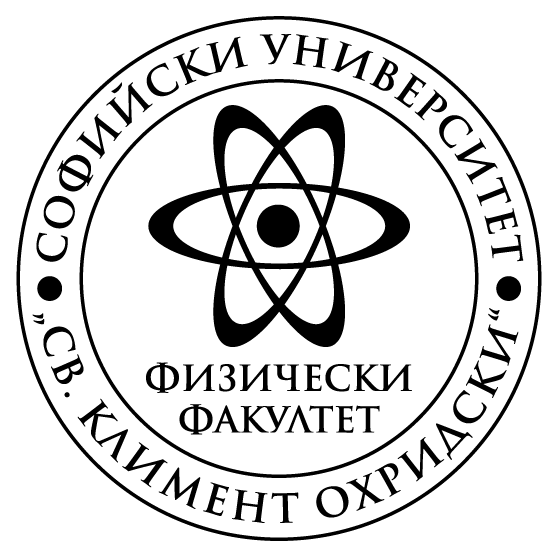
\includegraphics[scale = 0.5]{Pre-Defence/logo-FzF.png}
	\end{frame}
	
	% These three lines create an automatically generated table of contents.
	\begin{frame}{Outline}
		\tableofcontents
	\end{frame}
	
	\section{Предмет на дисертацията}
	
	\begin{frame}{Радио наблюдения на свръхмасивни компактни обекти}
		
		\centering
		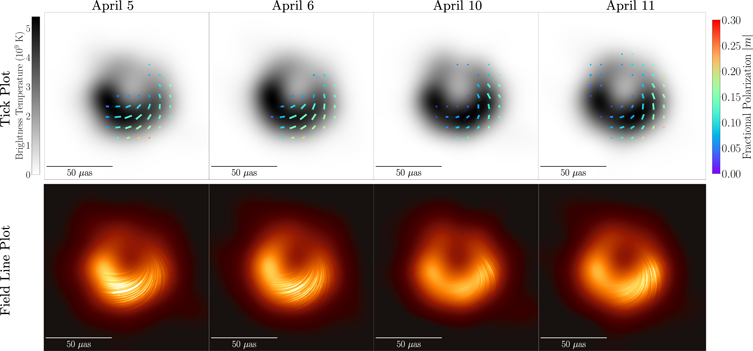
\includegraphics[scale = 0.4]{Pre-Defence/EHT_M87_pol.jpg}\\
		
		\tiny The Event Horizon Telescope Collaboration et al 2021 ApJL 910 L12
		
	\end{frame}
	
	\subsection{Отпечатъкът на пространство-времето върху радио наблюдения на свръхмасивни компактни обекти}
	
	\begin{frame}{Моделиране на М$87^*$ като екзотичен компактен обект}		
		
		\begin{block}{Допускаме следната хипотеза:}
			Наблюденията на EHT могат да
			бъдат възпроизведени от синхотронно излъчваща плазма, около свръхмасивни
			компактни обекти които \textbf{не} притежават хоризонт на събитията.
		\end{block}	
		
		\begin{center}
			$\downarrow$
		\end{center}
		\begin{alertblock}{Задаваме следният въпрос:}
			По какъв начин природата на пространство-времето се отпечатва върху получените чрез радио наблюдения образи?
		\end{alertblock}
		\begin{center}
			$\downarrow$
		\end{center}
		\begin{block}{Сравнителен анализ}
			Моделираме М87$^*$ като екзотичен компактен обект и симулираме неговите радио наблюдения.
		\end{block}
		
	\end{frame}
	
	\subsection{Публикации}
	
	\begin{frame}{Характеристики на наблюдаваните образи}
		\begin{block}{Природата на пространство-времето може (най-общо казано) да повлияе върху следните свойства на получените образи:}
			\centering
			$\bullet$ Морфологията\\
			$\bullet$ Поляризацията
			\begin{alertblock}{$ $}
				\centering
				$\bullet$ Променливостта
			\end{alertblock}
			
		\end{block}
		
		Променливостта, която за Sgr A$^*$ е значителна, се очаква да се влияе предимно от спецификите на акреционният поток, поради което \textbf{не} я разглеждаме в дисертацията.
		
	\end{frame}
	
	\begin{frame}{Публикации}
		
		\begin{block}{Публикации, разглеждащи морфологията}
			\small
			$\bullet$ V Deliyski, G Gyulchev, P Nedkova, and S Yazadjiev. Observational features
			of thin accretion disks around traversable wormholes. Journal of Physics:
			Conference Series, 2255(1):012002, apr 2022.\\
			$\bullet$ V Deliyski, G Gyulchev, P Nedkova, and S Yazadjiev.
			Observing naked singularities by the present and next-generation event horizon
			telescope. http://arxiv.org/abs/2401.14092, 2024.
		\end{block}
		
		\begin{block}{Публикации, разглеждащи поляризацията}
			\small
			$\bullet$ V Deliyski, G Gyulchev, P Nedkova, and S Yazadjiev.
			Polarized image of equatorial emission in horizonless spacetimes: Traversable
			wormholes. Phys. Rev. D, 106:104024, Nov 2022.\\
			$\bullet$ V Deliyski, G Gyulchev, P Nedkova, and S Yazadjiev.
			Polarized image of equatorial emission in horizonless spacetimes: Naked
			singularities. Phys. Rev. D, 108:104049, Nov 2023.
		\end{block}
		
	\end{frame}
	
	\section{Оптична проява на пространствено-времеви тунели}
	
	\begin{frame}{Оптична проява на пространствено-времеви тунели}		
		\tiny
		\begin{equation*}
			ds^2 = - N^2(r)dt^2 + \left(1- \frac{b}{r}\right)^{-1}dr^2 + r^2\left(d\theta^2 + \sin^2\theta d\phi^2\right), \quad N(r) = \exp\left(-\frac{r_0}{r} -\alpha \frac{r_0^2}{r^2}\right),\quad b = r_0
		\end{equation*}	
		\small
		\begin{block}{}
			Сферичната симетрия позволява извеждането на аналитичен критерий за съществуването на релативистки образи на даден източник.
		\end{block}	
		\begin{minipage}{25em}
			\tiny	
			\begin{equation}
				\begin{aligned}
				&\Delta\phi(\xi,r_s,r_\text{obs}) = \fint_{r_\text{obs}}^{r_\text{s}}\frac{dr}{\sqrt{-\frac{1}{\xi^2}\frac{g^2_{\phi\phi}}{g_{tt}g_{rr}}(1 - V_\text{eff})}},\quad V_\text{eff} = -\frac{g_{tt}}{g_{\phi\phi}}\xi^2
				\end{aligned}
			\end{equation}
			\begin{subequations}
				\begin{equation}
					\begin{aligned}
						&\delta_n(\xi_n,r_s,r_\text{obs}) = \arcsin\left[\frac{\cot\left(\Delta\phi(\xi_n,r_s,r_\text{obs}) - n\pi\right)}{\tan i}\right]\\
						&\sigma_n(\xi_n,r_s,r_\text{obs}) = \arcsin\left[\xi_n\sqrt{-\frac{g_{tt}}{g_{\phi\phi}}}\right]\bigg\vert_{r = r_\text{obs}}
					\end{aligned}
				\end{equation}
				\begin{equation}
					\boxed{x_n = \sqrt{g_{\phi\phi}}\vert_{r=r_\text{obs}}\sigma_n\cos\delta_n,\,\,\,y_n = \sqrt{g_{\phi\phi}}\vert_{r=r_\text{obs}}\sigma_n\sin\delta_n}
				\end{equation}
			\end{subequations}
		\end{minipage}
		\begin{minipage}{6em}
			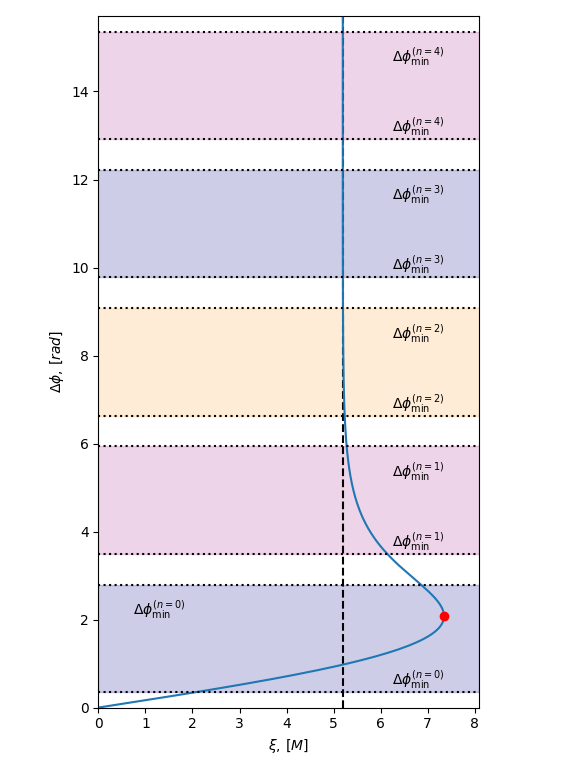
\includegraphics[scale = 0.2]{Section_6_Morphology_of_the images_of_horizonless_spacetimes/Schw_70_deg_ISCO_impact.png}
		\end{minipage}
				
	\end{frame}
	
	\begin{frame}{Оптична проява на пространствено-времеви тунели}		
		\centering
		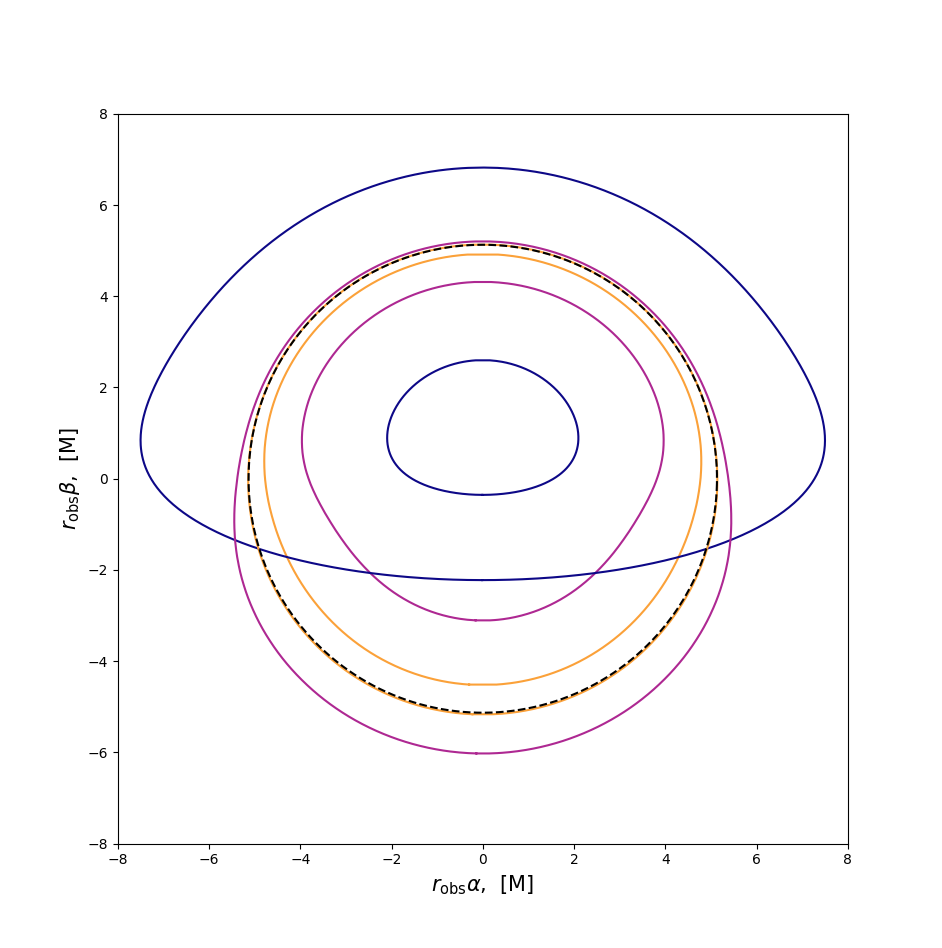
\includegraphics[scale = 0.2]{Section_6_Morphology_of_the images_of_horizonless_spacetimes/WH_70_deg_r6_gamma_2.png}
		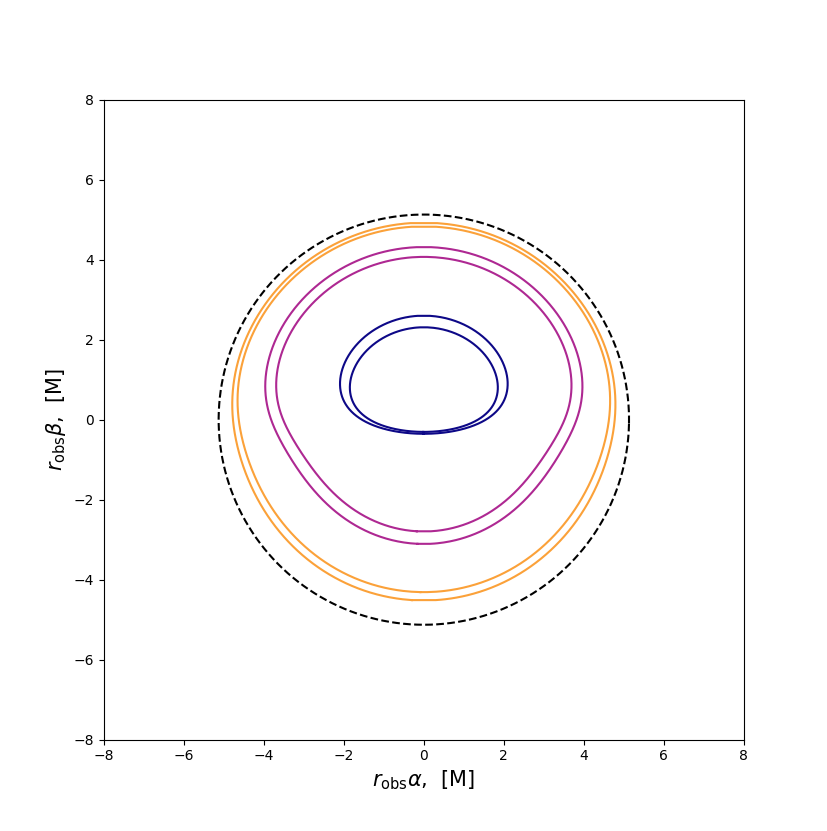
\includegraphics[scale = 0.2]{Section_6_Morphology_of_the images_of_horizonless_spacetimes/WH_70_deg_r6_r500.png}
		
		\tiny V Deliyski, G Gyulchev, P Nedkova, and S Yazadjiev. Observational features
		of thin accretion disks around traversable wormholes. Journal of Physics:
		Conference Series, 2255(1):012002, apr 2022.
	\end{frame}
	
	\subsection{Наблюдателна значимост на екзотичните образи}
	
	\begin{frame}{Наблюдателна значимост на екзотичните образи}

		\centering
		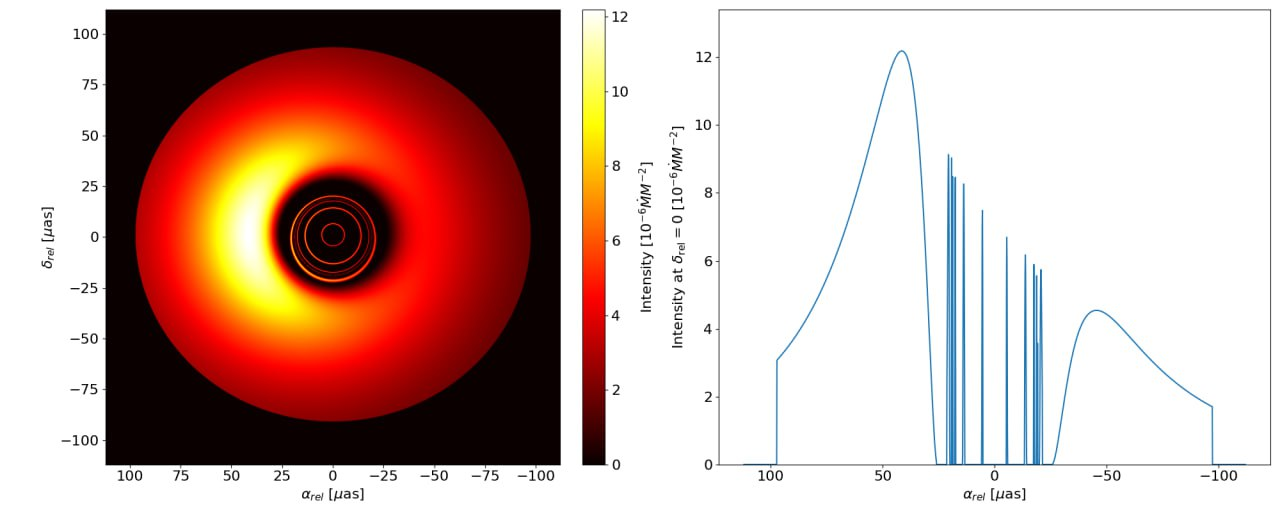
\includegraphics[scale = 0.3]{Pre-Defence/WH_20_deg.jpg}
		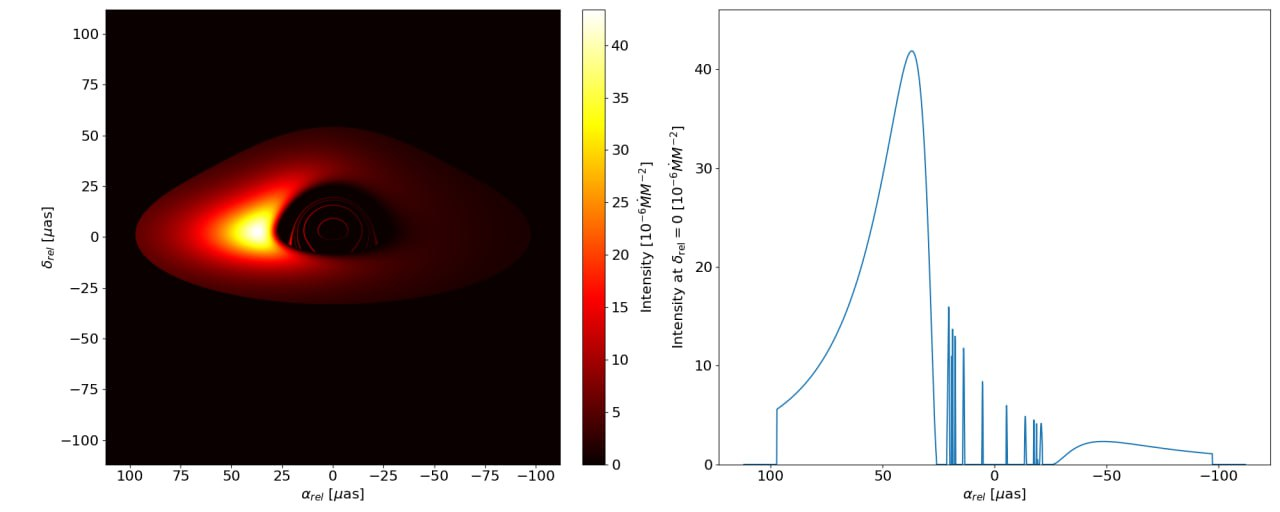
\includegraphics[scale = 0.3]{Pre-Defence/WH_70_deg.jpg}

		
	\end{frame}
	
	\section{Отпечатък на пространство-времето върху поляризацията на образите}
	
	\begin{frame}{Отпечатък на пространство-времето върху поляризацията на образите}
		\begin{block}{Природа да поляризираното лъчение}
			Наблюденията на M87$^*$ и Sgr A$^*$ се описват добре от високо-температурна и оптически тънка плазма, излъчваща синхотронно.
		\end{block}
		
		\begin{center}
			$\downarrow$
		\end{center}
		
		\begin{block}{Метод на анализ}
			Използваме опростен модел на излъчващият механизъм, който се възползва от Килинговите симетрии на пространство-времето за да пресметне наблюдаваната на безкрайност поляризация.
		\end{block}
	\end{frame}
	
	\begin{frame}{Модел на поляризираното излъчване}
		\small
		\begin{block}{}
			Моделът се възползва от съществуването на тензор на Килинг-Яно (за разгледаните от нас пространства) $Y_{\mu\nu}$, и дуалният му $\tilde{Y}_{\mu\nu} = \frac{1}{2}\epsilon_{\mu\nu\alpha\beta}Y^{\alpha\beta}$.
		\end{block}
		
		\tiny
		\noindent
		\centering{
		\begin{minipage}{18em}
			\begin{subequations}
				\begin{equation}
					\kappa_1 = \frac{1}{2}\tilde{Y}_{\mu\nu}p^\mu f^\nu = \text{const}
				\end{equation}
				\vspace{1mm}
				\begin{equation}
					\kappa_2 = {Y}_{\mu\nu}p^\mu f^\nu = \text{const}
				\end{equation}
			\end{subequations}
		\end{minipage}
		$\qquad\large\rightarrow$
		\begin{minipage}{14em}
			\vspace{1mm}
			\begin{subequations}
				\begin{equation}
					f^x = \frac{x\kappa_1 + y\kappa_2}{x^2 + y^2}
				\end{equation}
				\begin{equation}
					f^y = \frac{y\kappa_1 - x\kappa_2}{x^2 + y^2}
				\end{equation}
			\end{subequations}
		\end{minipage}}
		\hspace{10cm}
		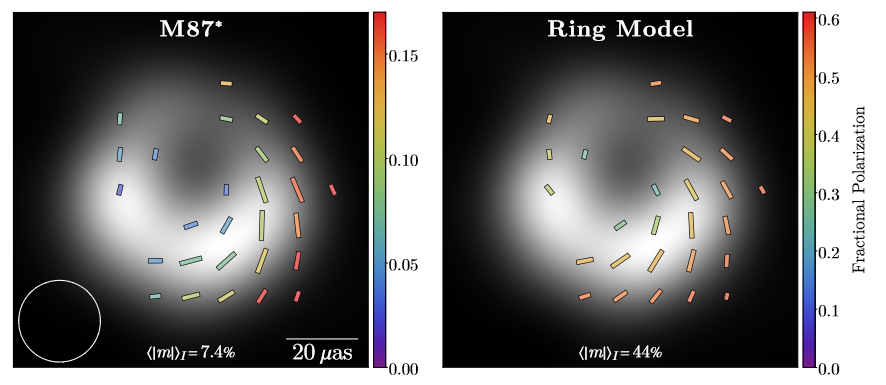
\includegraphics[scale = 0.4]{Pre-defence/M87_model_comparison.png}\\
		\tiny
		R. Narayan, D. C. M. Palumbo, M. D. Johnson, Z. Gelles, E. Himwich, D. O. Chang, A. Ricarte, J. Dexter, C. F. Gammie, A. A. Chael, and The Event Horizon Telescope Collaboration, “The Polarized Image of a Synchrotron-emitting Ring of Gas Orbiting a Black Hole,” The Astrophysical Journal 912 no. 1, (May, 2021)
	\end{frame}
	
	\begin{frame}{Поляризационни свойства на екзотични компактни обекти - директни образи}
		\centering
		\centering{\small Пространствено-времеви тунел}
		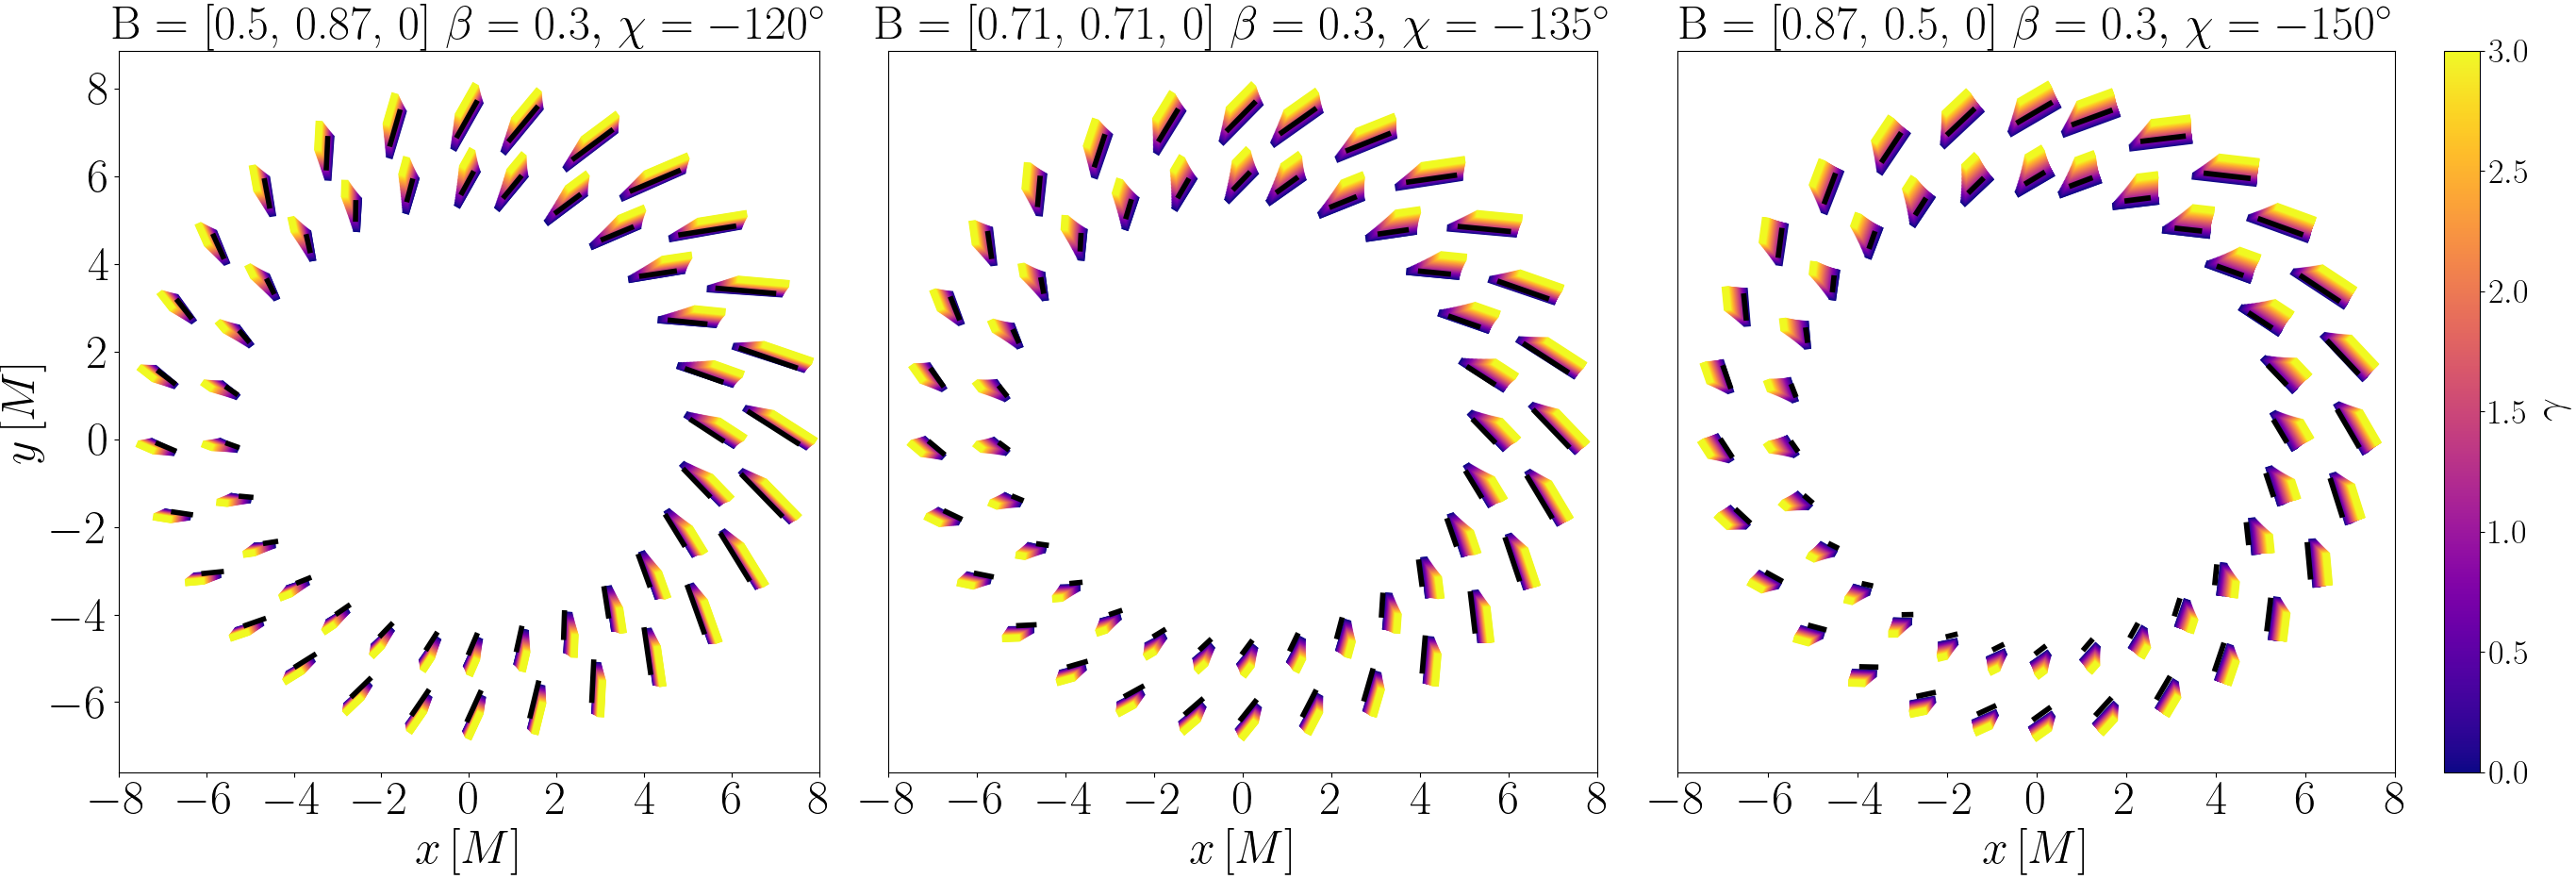
\includegraphics[scale = 0.14]{Section_7_Polarized_Emission/WH_alpha_Eq_Field.png}\\
		\centering{\small Гола сингуларност на Джанис-Нюман-Уиникър}
		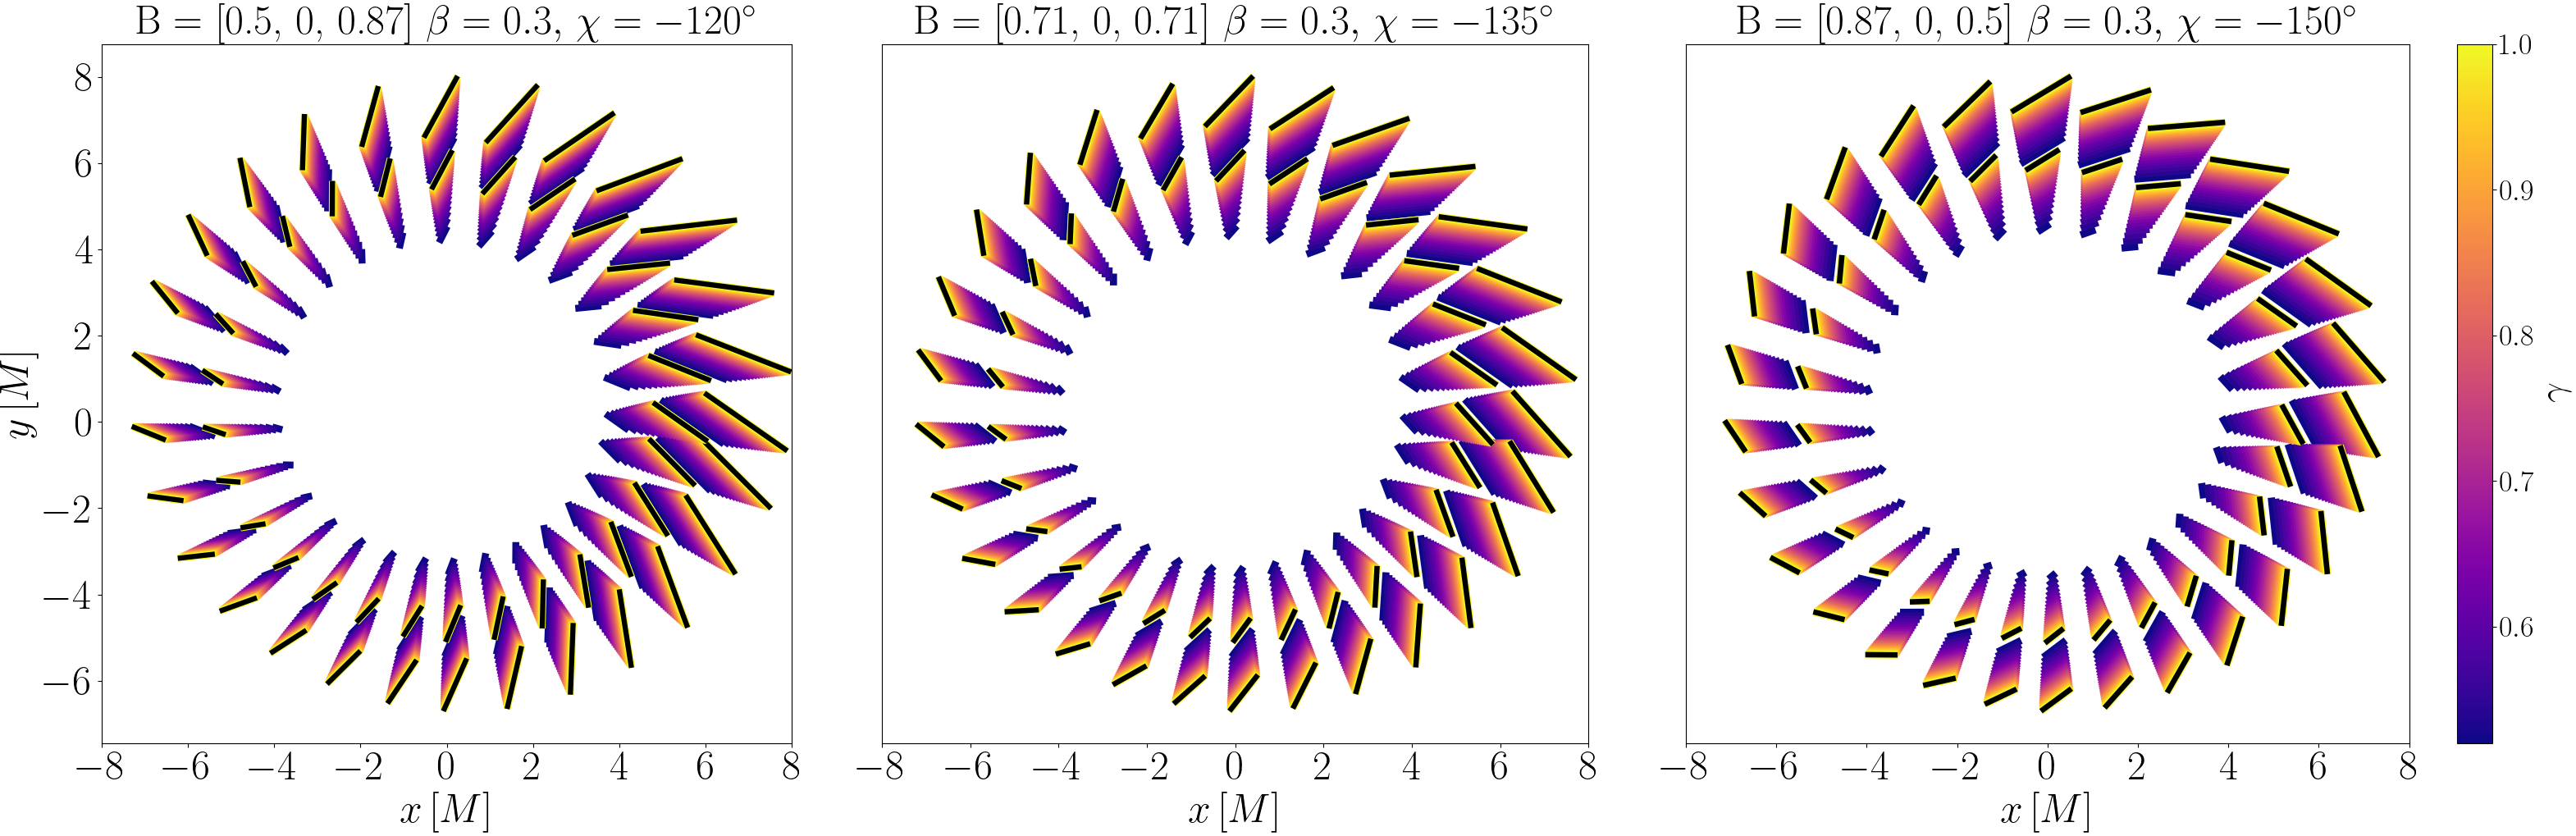
\includegraphics[scale = 0.12]{Section_7_Polarized_Emission/JNW_alpha_Eq_Field.png}
	\end{frame}
	
	\begin{frame}{Поляризационни свойства на екзотични компактни обекти - индиректни образи}
		
		\centering
		\centering{\small Пространствено-времеви тунел}
		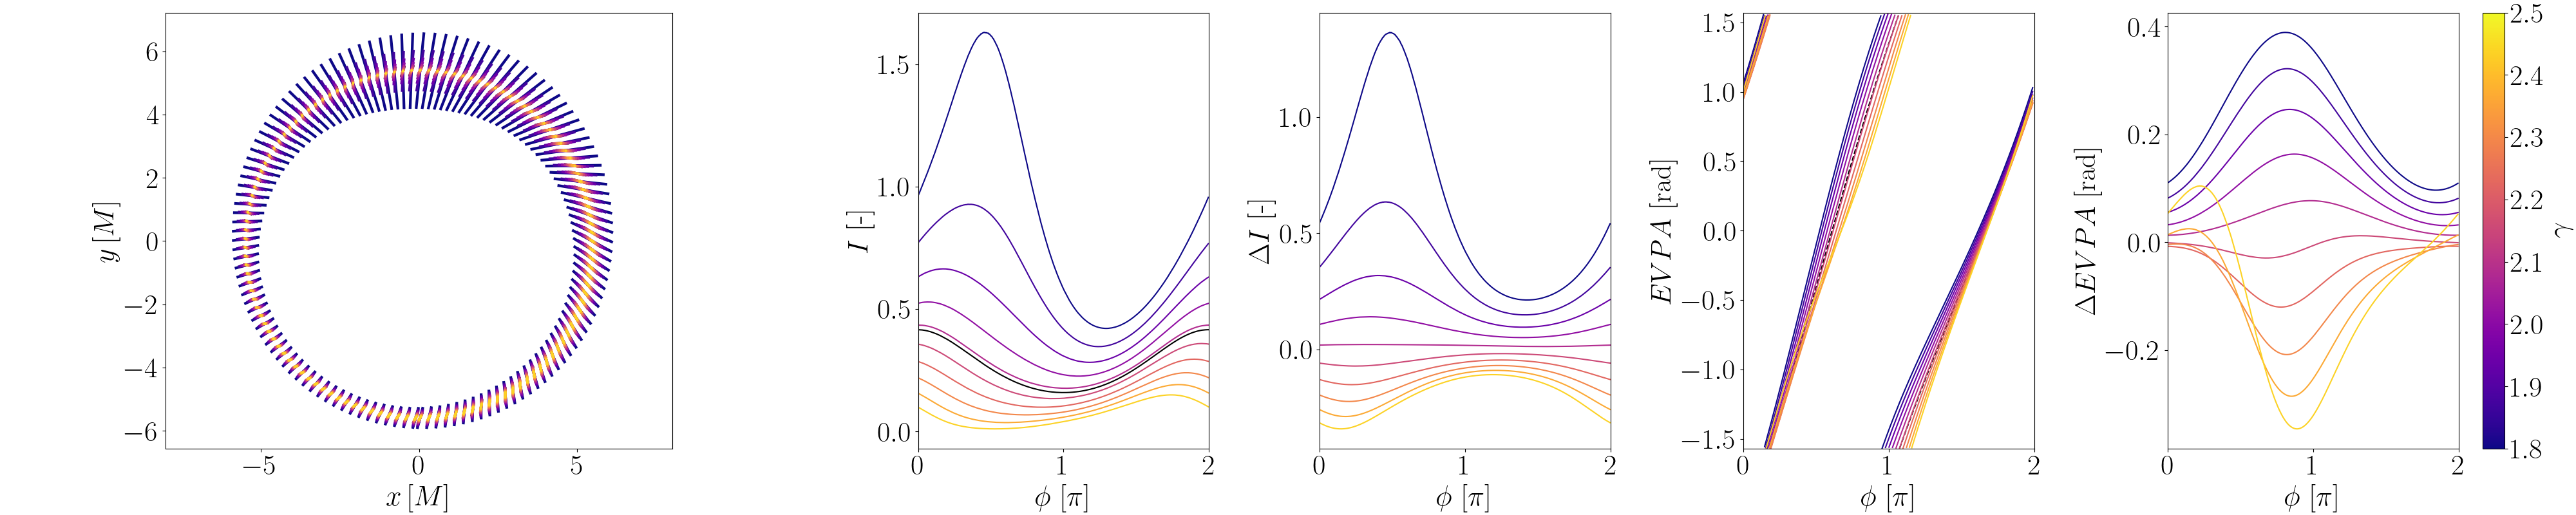
\includegraphics[scale = 0.12]{Section_7_Polarized_Emission/WH_delta_fig_B_0.5_0.87_0_20_deg_r6_n1.png}
		\centering{\small Гола сингуларност на Джанис-Нюман-Уиникър}
		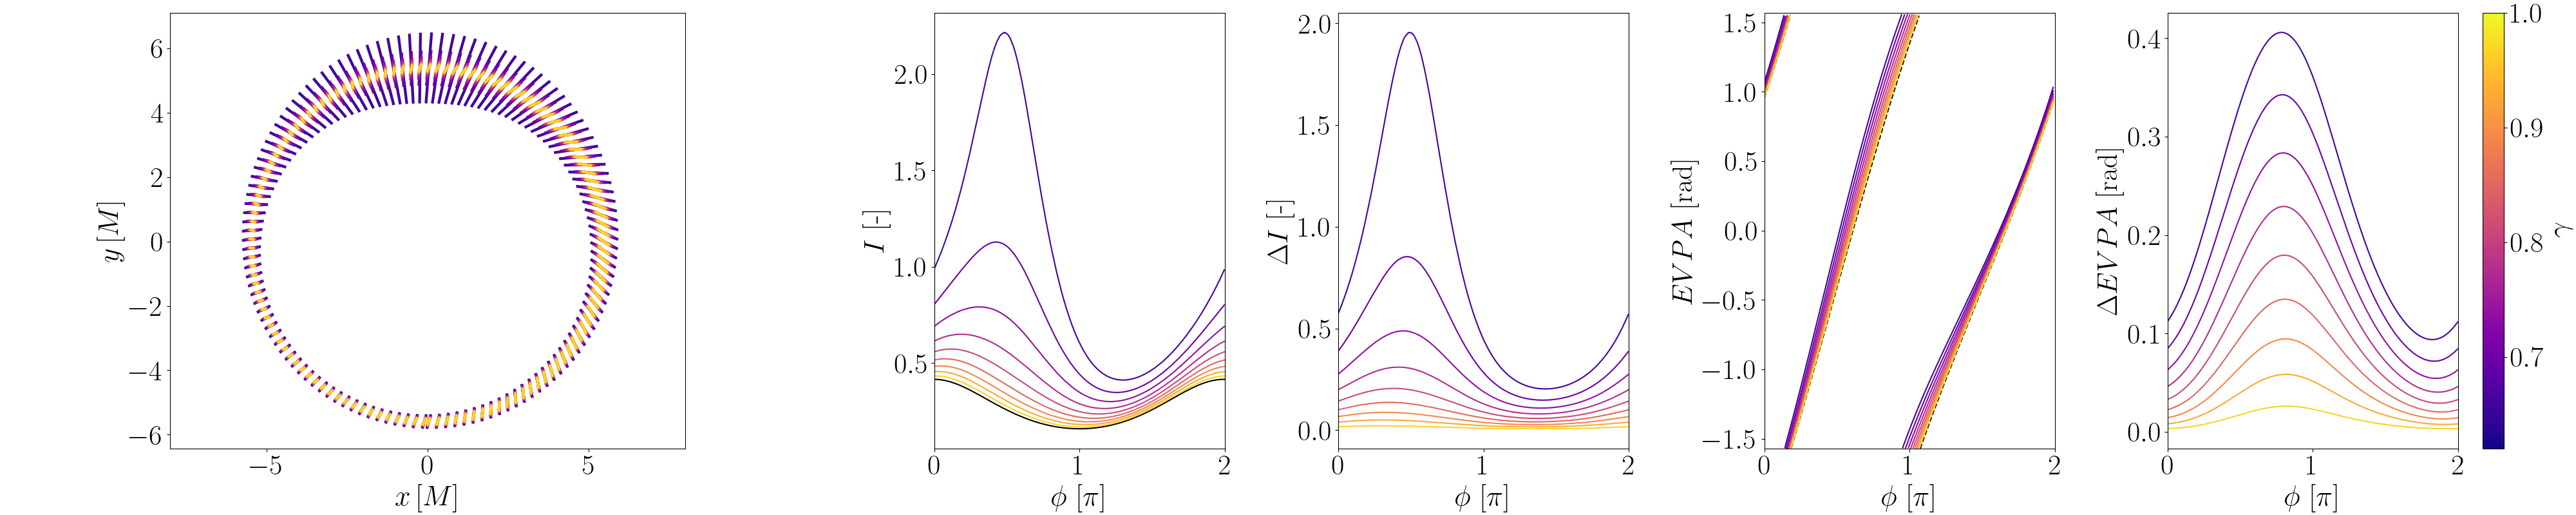
\includegraphics[scale = 0.12]{Section_7_Polarized_Emission/JNW_delta_fig_B_0.5_0.87_0_20_deg_r6_n1.png}\\
		
			
		\tiny  $\bullet$ V Deliyski, G Gyulchev, P Nedkova, and S Yazadjiev.
		Polarized image of equatorial emission in horizonless spacetimes: Traversable
		wormholes. Phys. Rev. D, 106:104024, Nov 2022.\\
		$\bullet$ V Deliyski, G Gyulchev, P Nedkova, and S Yazadjiev.
		Polarized image of equatorial emission in horizonless spacetimes: Naked
		singularities. Phys. Rev. D, 108:104049, Nov 2023.
		
	\end{frame}

	
	\section{Наблюдения на екзотични компактни обекти от ngEHT}
	
	\subsection{VLBI наблюдения}
	
	\begin{frame}{VLBI наблюдения}

		\centering
		\qquad
		\begin{minipage}{11em}
			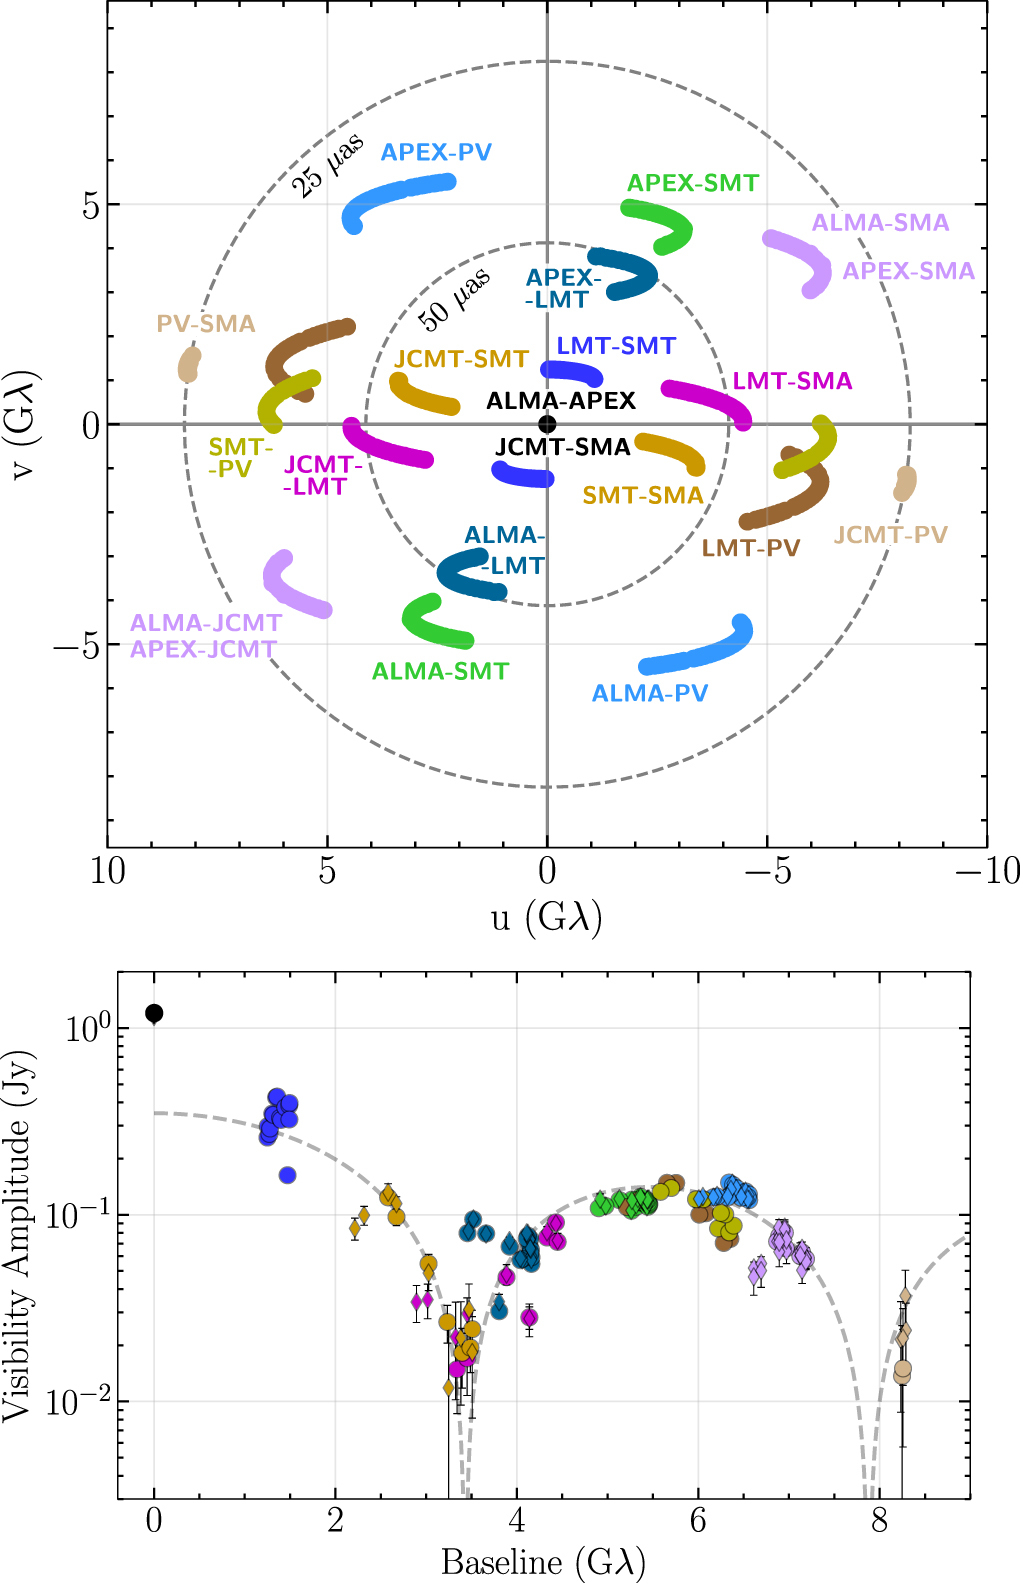
\includegraphics[scale = 0.5]{Pre-Defence/UV_coverage.jpg}
		\end{minipage}\,\,\,\huge$\rightarrow$
		\begin{minipage}{8em}
			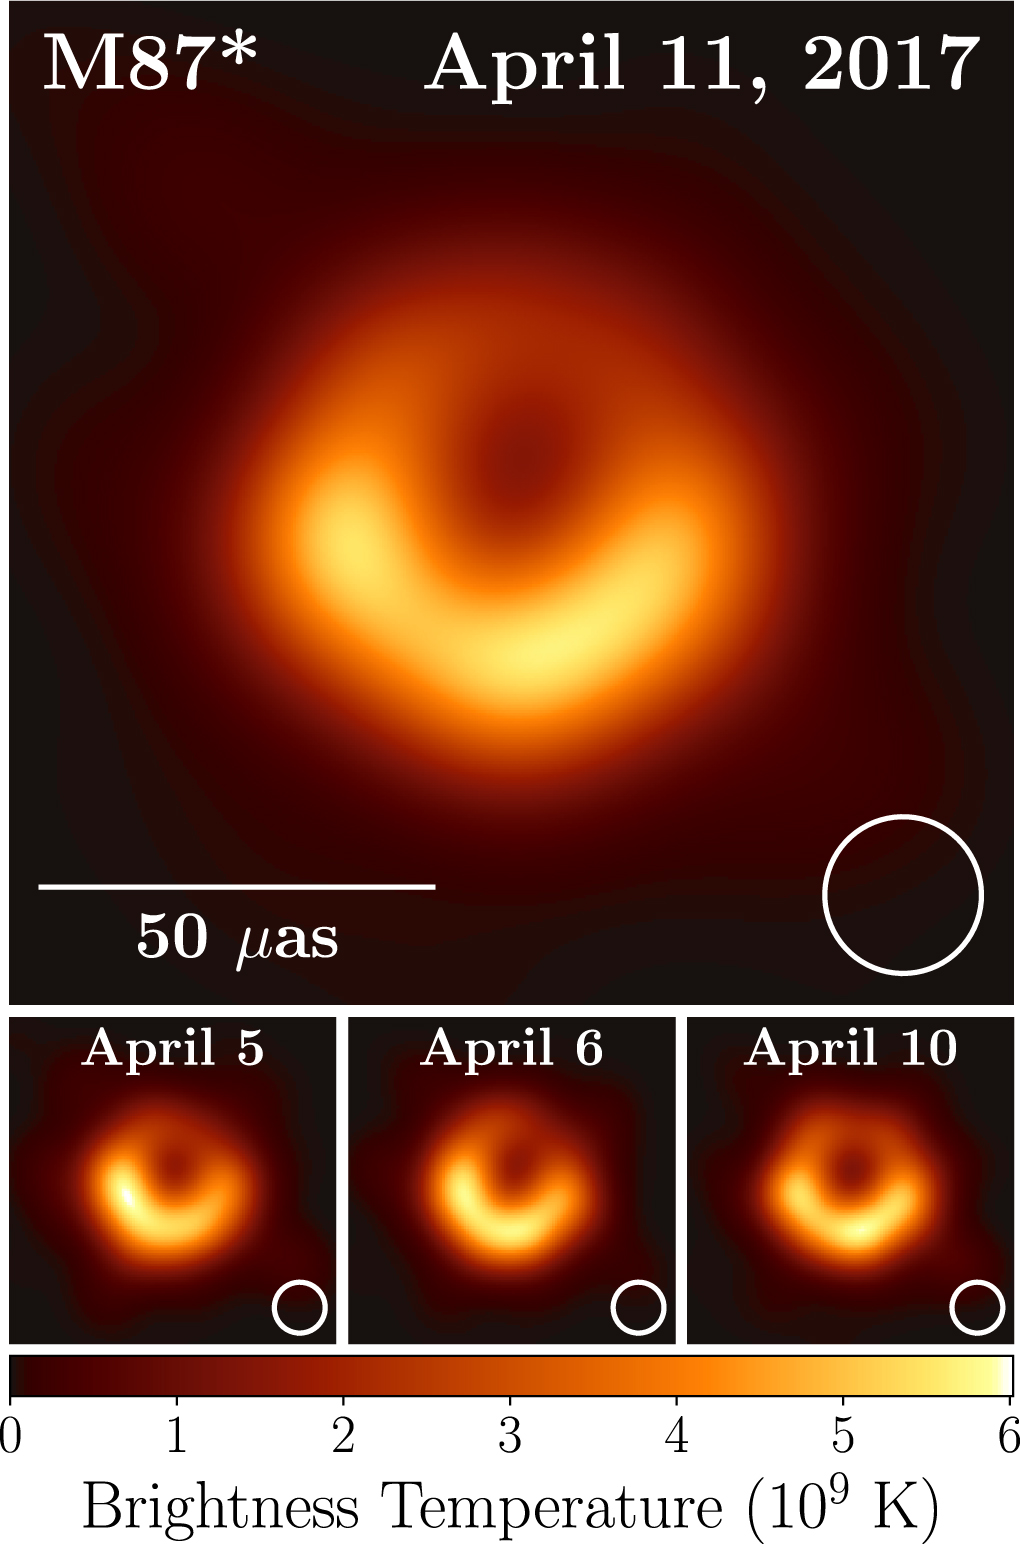
\includegraphics[scale = 0.5]{Pre-Defence/M87.jpg}
		\end{minipage}\\
		
		\tiny The Event Horizon Telescope Collaboration et al 2019 ApJL 875 L1
		
	\end{frame}
	
	\subsection{Методика за симулиране на VLBI наблюдения}
	
	\begin{frame}{Методика за симулиране на VLBI наблюдения}
		
		\begin{block}{Генериране на "идеално"$\,$ наблюдение}
			\small
			\begin{subequations}
				\begin{equation*}
					\frac{dx^\mu}{d\lambda} = \frac{\partial H}{\partial k_\mu},\quad \frac{d k_\mu}{d\lambda} = - \frac{\partial H}{\partial x^\mu},
				\end{equation*}
				\begin{equation*}
					k^\nu\nabla_\nu f^\mu = 0,
				\end{equation*}
				\begin{equation*}
					\frac{d}{d\lambda} \begin{pmatrix}
						\mathcal{I}_\nu\\
						\mathcal{Q}_\nu\\
						\mathcal{U}_\nu\\
						\mathcal{V}_\nu
					\end{pmatrix} = 
					\begin{pmatrix}
						\mathcal{J}_\mathcal{I,\nu}\\
						\mathcal{J}_\mathcal{Q,\nu}\\
						\mathcal{J}_\mathcal{U,\nu}\\
						\mathcal{J}_\mathcal{V,\nu}
					\end{pmatrix}
					-	\begin{pmatrix}
						\kappa_\mathcal{I,\nu} & \kappa_\mathcal{Q,\nu} & \kappa_\mathcal{U,\nu} & \kappa_\mathcal{V,\nu}\\
						\kappa_\mathcal{Q,\nu}& \kappa_\mathcal{I,\nu}& -\rho_\mathcal{U,\nu}& \rho_\mathcal{V,\nu}\\     	
						\kappa_\mathcal{U,\nu}& -\rho_\mathcal{V,\nu}& \kappa_\mathcal{I,\nu}& \rho_\mathcal{Q,\nu}\\	  
						\kappa_\mathcal{V,\nu}& \rho_\mathcal{U,\nu}& -\rho_\mathcal{Q,\nu}& \kappa_\mathcal{I,\nu}\\
					\end{pmatrix}
					\begin{pmatrix}
						\mathcal{I}_\nu\\
						\mathcal{Q}_\nu\\
						\mathcal{U}_\nu\\
						\mathcal{V}_\nu
					\end{pmatrix}
				\end{equation*}
			\end{subequations}
			
		\end{block}
		
		\centering
		\includegraphics[scale = 0.35]{Pre-Defence/github.png}
		\tiny https://github.com/ValentinDeliyski/Mjolnir\_GRRT/tree/develop
	\end{frame}
	
	\begin{frame}{Генериране на "идеално"$\,$ наблюдение}
		\centering
		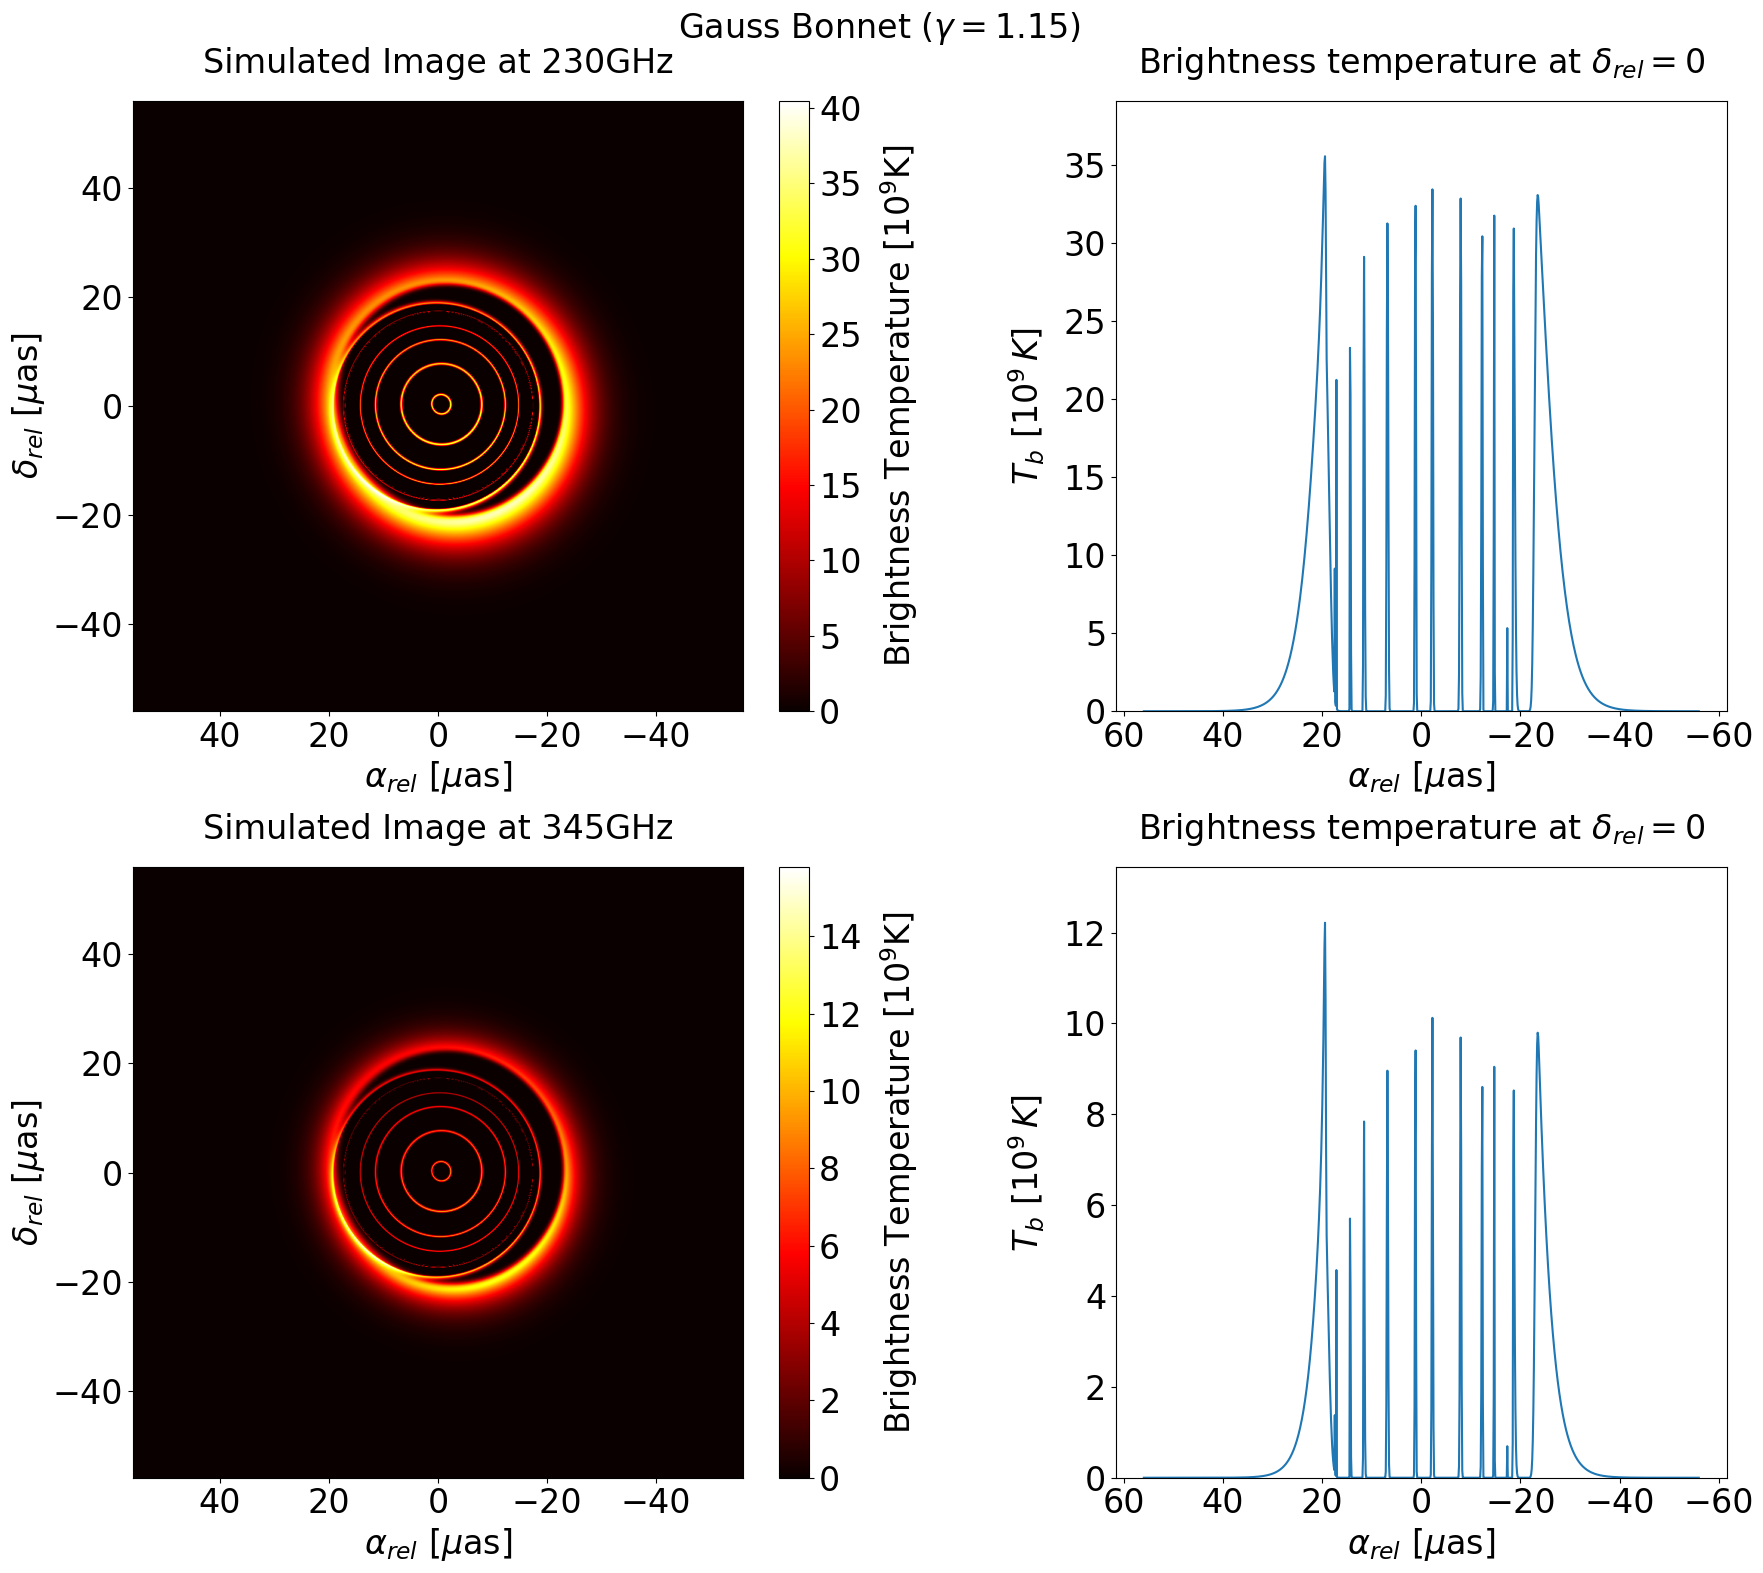
\includegraphics[scale = 0.18]{Pre-Defence/Ray_tracer_plot_230_345.png}\\
		
		\tiny V. Deliyski, G. Gyulchev, P. Nedkova, and S. Yazadjiev. Observing naked singularities
		by the present and next-generation event horizon telescope. [arXiv:2401.14092 [gr-qc]].
	\end{frame}
	
	\begin{frame}{Генериране на реално наблюдение с пакета \textbf{ehtim}}
			\centering
		\begin{minipage}{13em}
			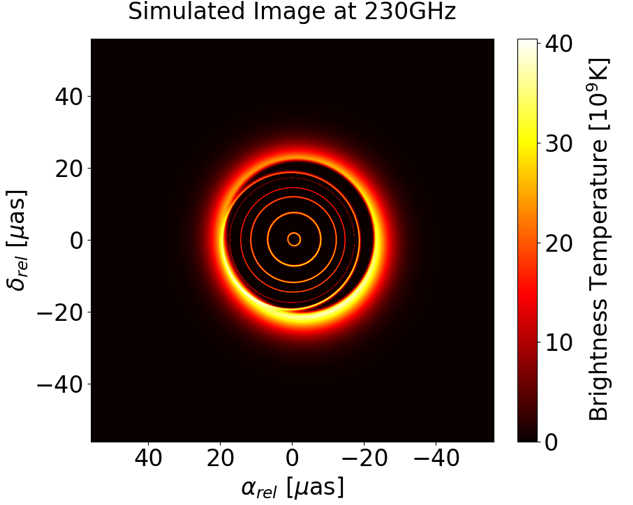
\includegraphics[scale = 0.50]{Pre-Defence/GB_ray_tracer_230.png}
		\end{minipage}\qquad$\rightarrow$
		\begin{minipage}{13em}
			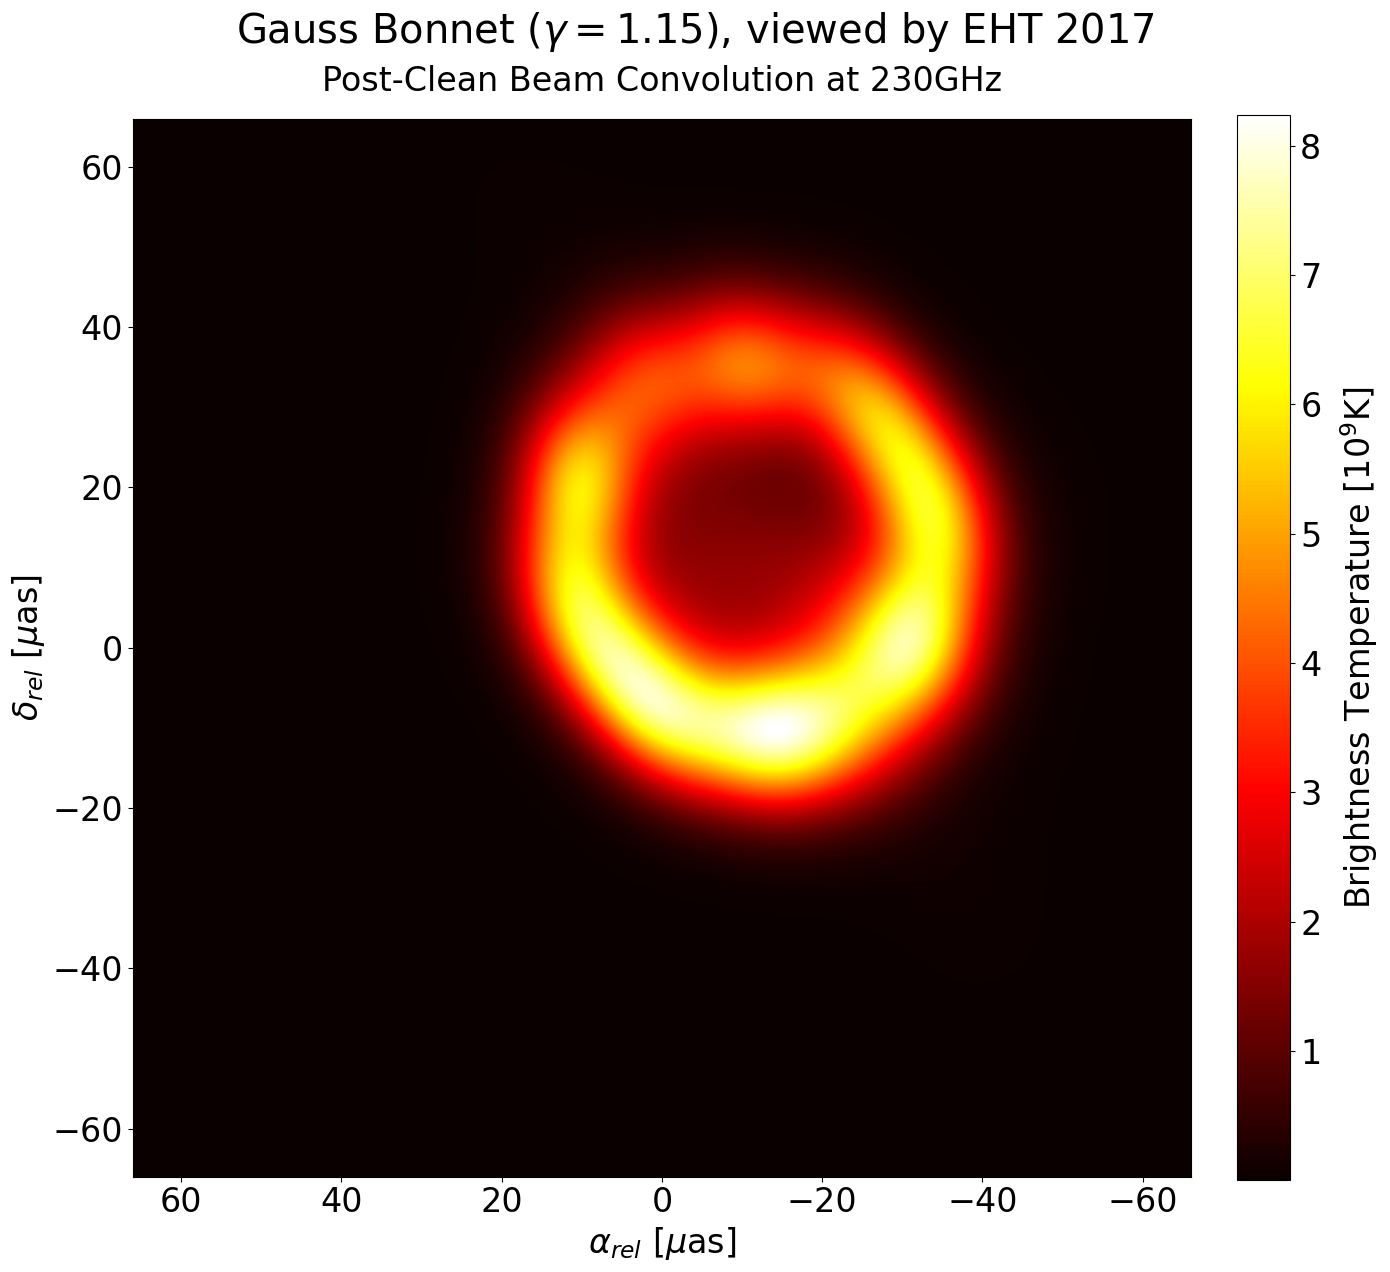
\includegraphics[scale = 0.14]{Pre-Defence/Ehtim_plot_2017.png}
		\end{minipage}\\
		
		\tiny V. Deliyski, G. Gyulchev, P. Nedkova, and S. Yazadjiev. Observing naked singularities
		by the present and next-generation event horizon telescope. [arXiv:2401.14092 [gr-qc]].\\
		
		
\includegraphics[scale = 0.35]{Pre-Defence/ehtim_github.png}
		\tiny https://github.com/achael/eht-imaging
	\end{frame}
	
	\begin{frame}{Генериране на реално наблюдение с пакета \textbf{ehtim}}
		\centering
		\begin{minipage}{13em}
			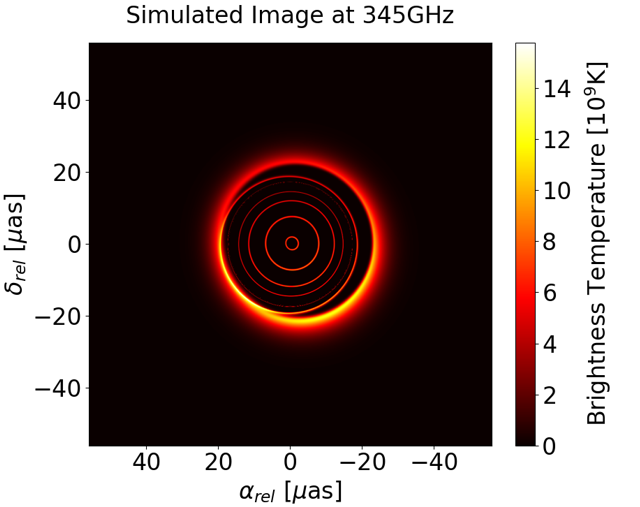
\includegraphics[scale = 0.50]{Pre-Defence/GB_ray_tracer_345.png}
		\end{minipage}\qquad$\rightarrow$
		\begin{minipage}{13em}
			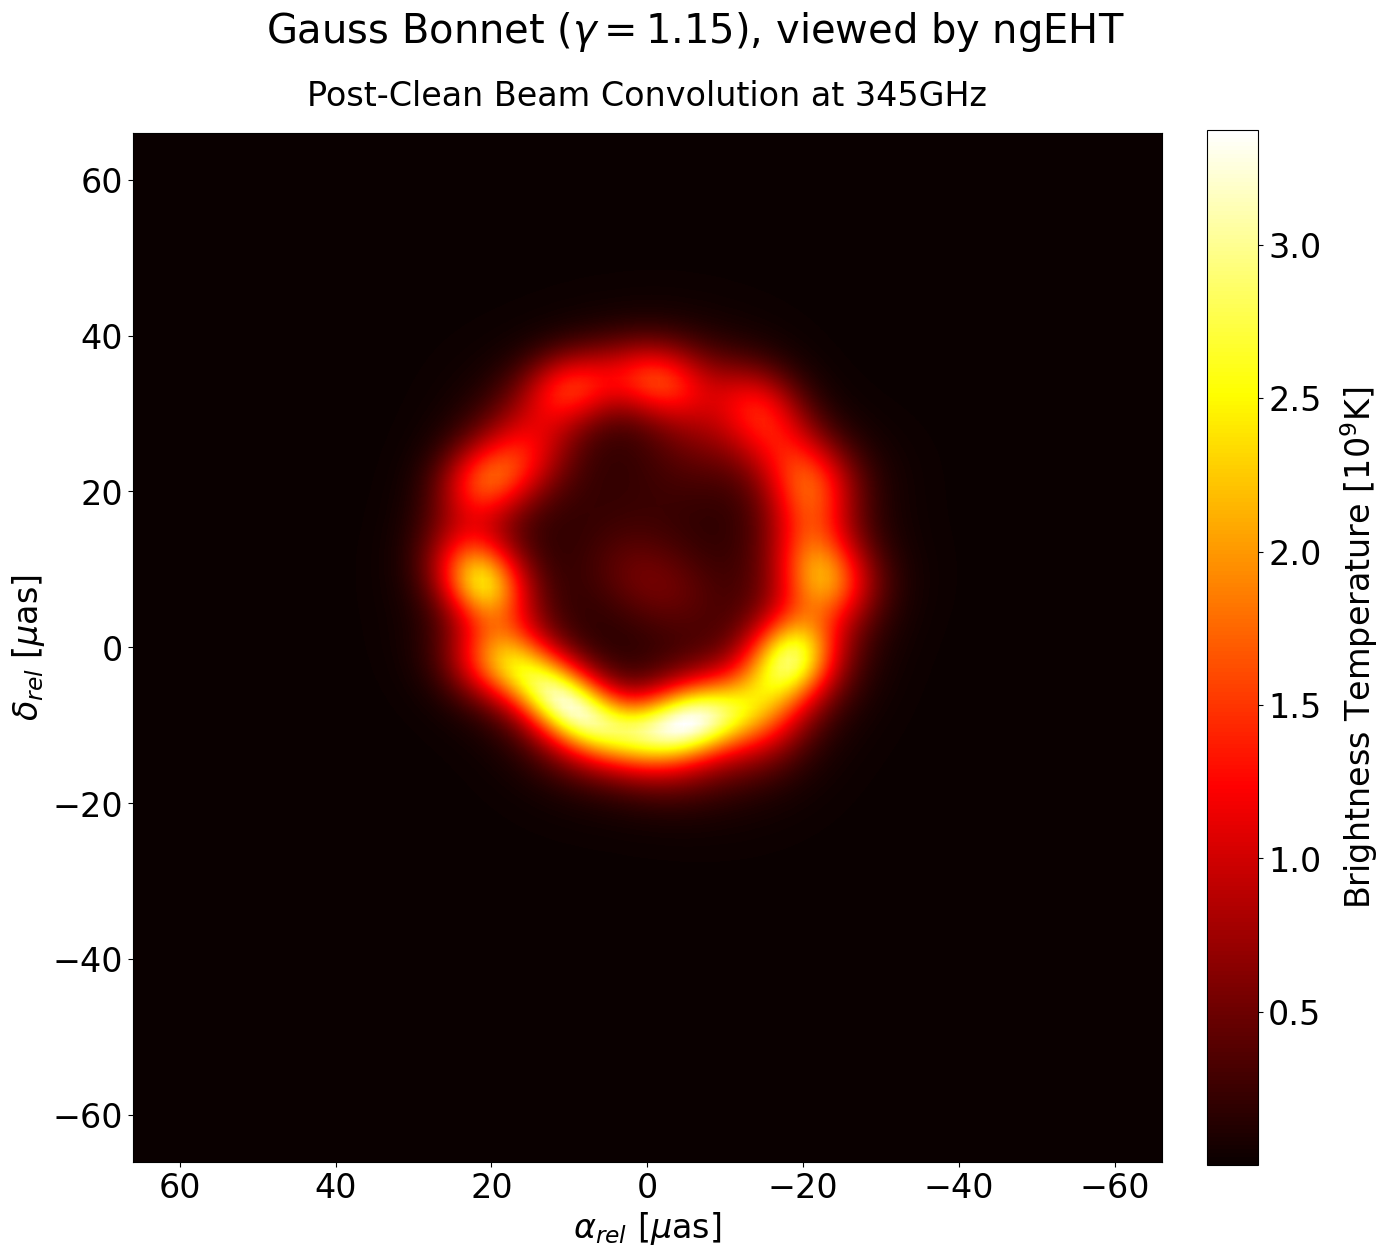
\includegraphics[scale = 0.14]{Pre-Defence/Ehtim_plot_ngEHT_345.png}
		\end{minipage}\\
		
		\tiny V Deliyski, G Gyulchev, P Nedkova, and S Yazadjiev.
		Observing naked singularities by the present and next-generation event horizon
		telescope. http://arxiv.org/abs/2401.14092, 2024.
	\end{frame}
	
	\begin{frame}{Морфологичен анализ на образите с пакета \textbf{VIDA}}
		
		\centering
		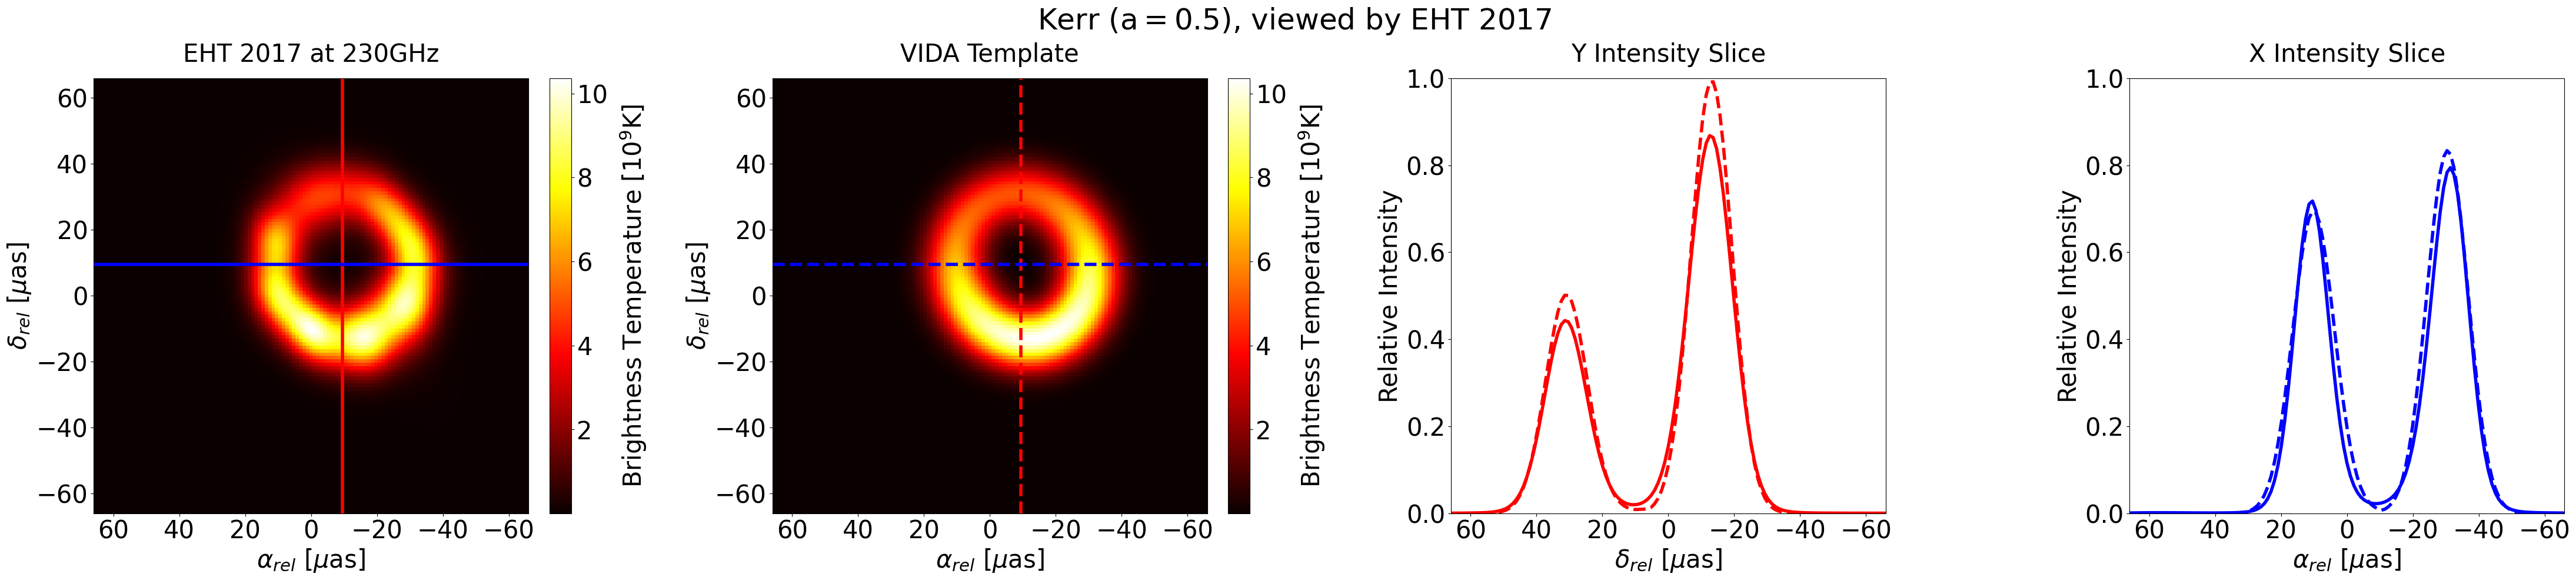
\includegraphics[scale = 0.11]{Pre-Defence/Ehtim_Vida_plot_2017_230_Kerr.png}\\
		\tiny V. Deliyski, G. Gyulchev, P. Nedkova, and S. Yazadjiev. Observing naked singularities
		by the present and next-generation event horizon telescope. [arXiv:2401.14092 [gr-qc]].\newline
	
		
\includegraphics[scale = 0.35]{Pre-Defence/VIDA_github.png}
		\tiny https://github.com/ptiede/VIDA.jl
		%Количествена оценка за морфологията даваме с $f_c = \frac{\min\mathcal{F}_{\text{center}}}{\langle{\mathcal{F}}_{\text{ring}}\rangle}$\\
		%При 230 GHz $f_{c,\text{Kerr}} \approx 10^{-2} - 10^{-3}$, $f_{c,\text{GB}} > 10^{-1} $\\

	\end{frame}
	
	\begin{frame}{Морфологичен анализ на образите с пакета \textbf{VIDA}}
		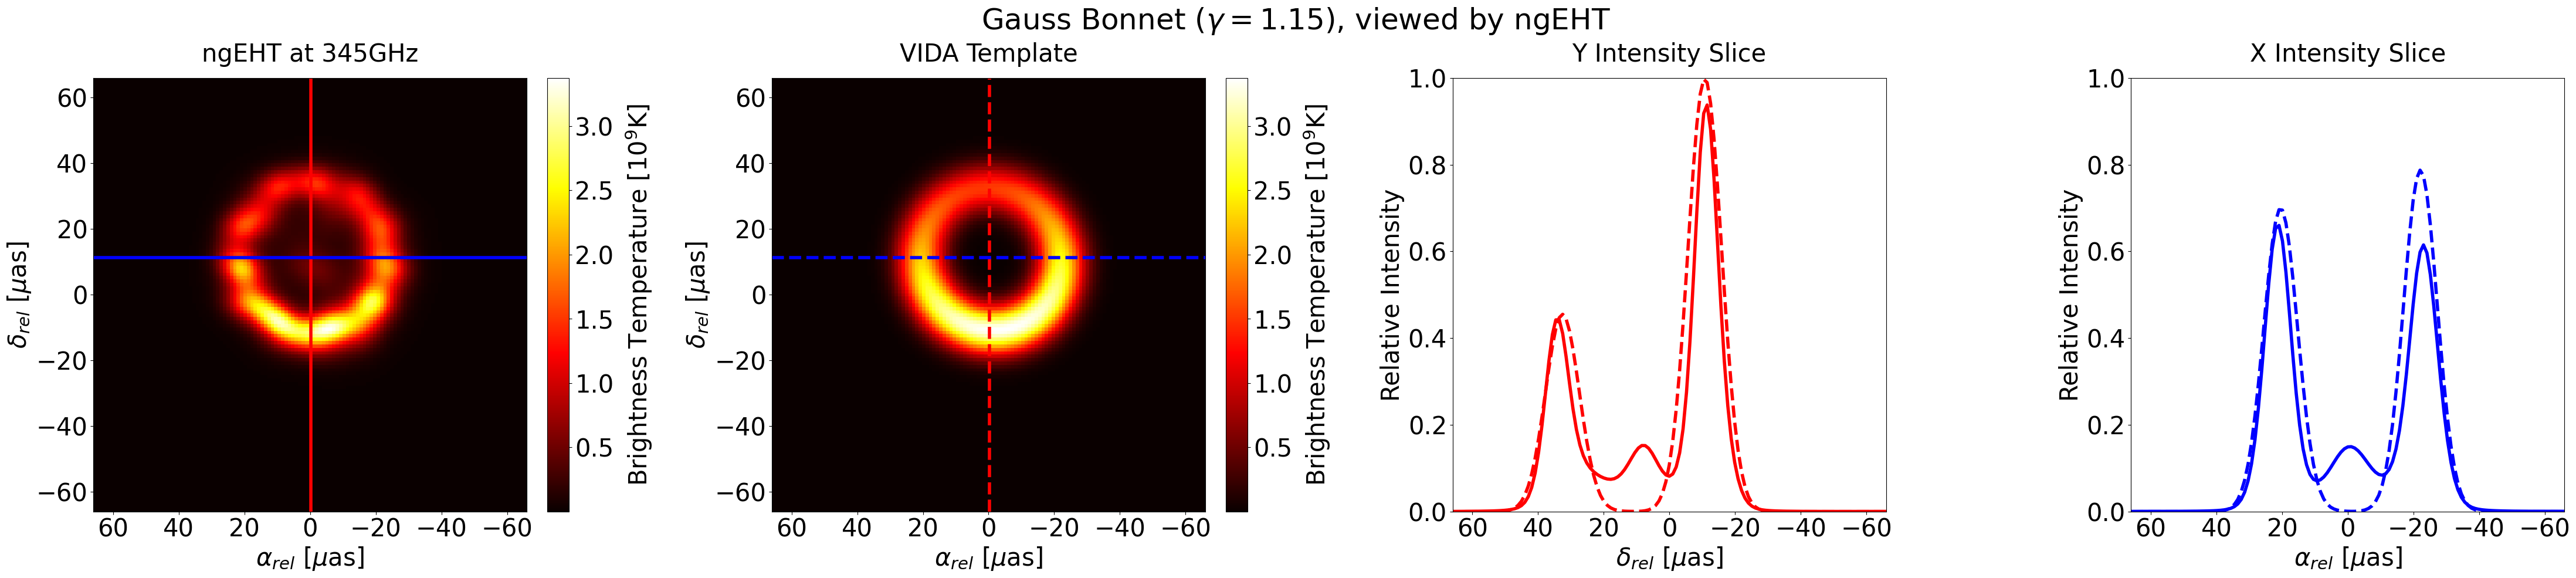
\includegraphics[scale = 0.11]{Pre-Defence/Ehtim_Vida_plot_ngEHT_345.png}\\
		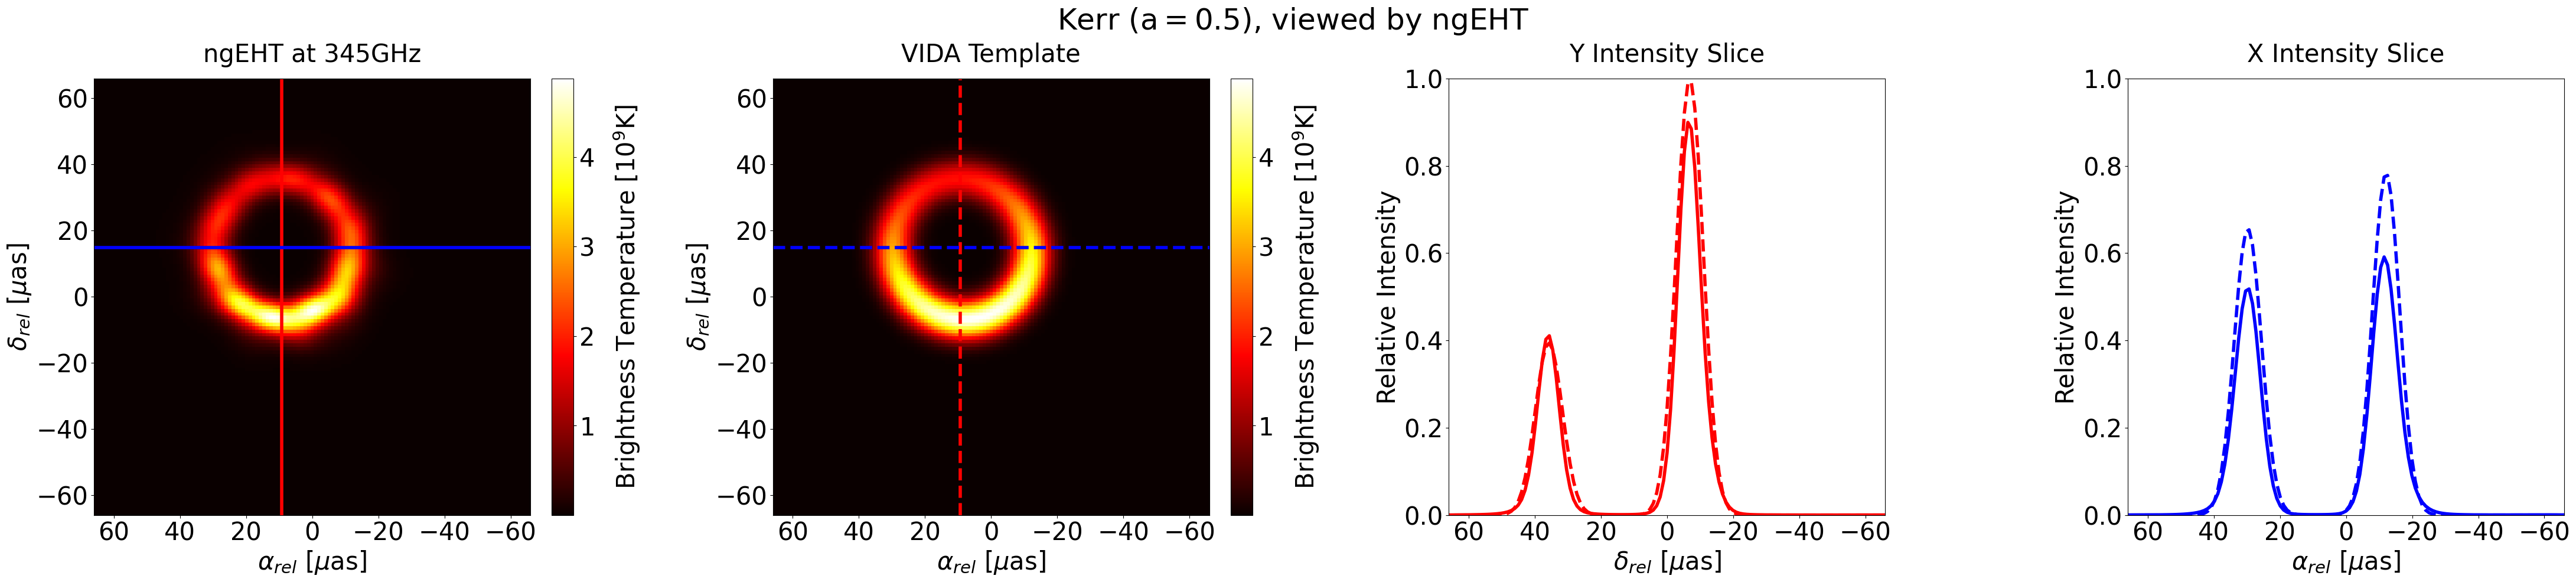
\includegraphics[scale = 0.11]{Pre-Defence/Ehtim_Vida_plot_ngEHT_345_kerr.png}\newline
		\tiny V. Deliyski, G. Gyulchev, P. Nedkova, and S. Yazadjiev. Observing naked singularities by the present and next-generation event horizon telescope. [arXiv:2401.14092 [gr-qc]].\\

	\end{frame}
	
	\begin{frame}{Морфологичен анализ на образите с пакета \textbf{VIDA}}
		\small
		\begin{block}{Количествена оценка за присъствието на централни пръстени}
			Използвайки темплейта въвеждаме мярката $\hat{f}_c = \frac{\min\mathcal{F}_{\text{center}}}{\langle{\mathcal{F}}_{\text{ring}}\rangle}$.
		\end{block}
		\tiny
		\begin{table}
			\centering
			\begin{tabular}{||c|c|c|c|c||}
				\hline
				{Metric} & {Schwarzschild}&{Kerr (a=0.5)}&{Gauss-Bonnet}&{J.N.W.}
				\\\hline
				{{$\hat{f}_c$ 230 GHz}} & 0.007&0.007&0.21&0.354
				\\\hline
				{{$\hat{f}_c$ 345 GHz}} & 0.002&0.002&0.12&0.220
				\\\hline
				{{$\hat{f}_c$ 230 GHz $\cup$ 345 GHz}} & 0.005&0.005&0.20&0.344
				\\\hline
			\end{tabular}
		\end{table}	
		\centering
		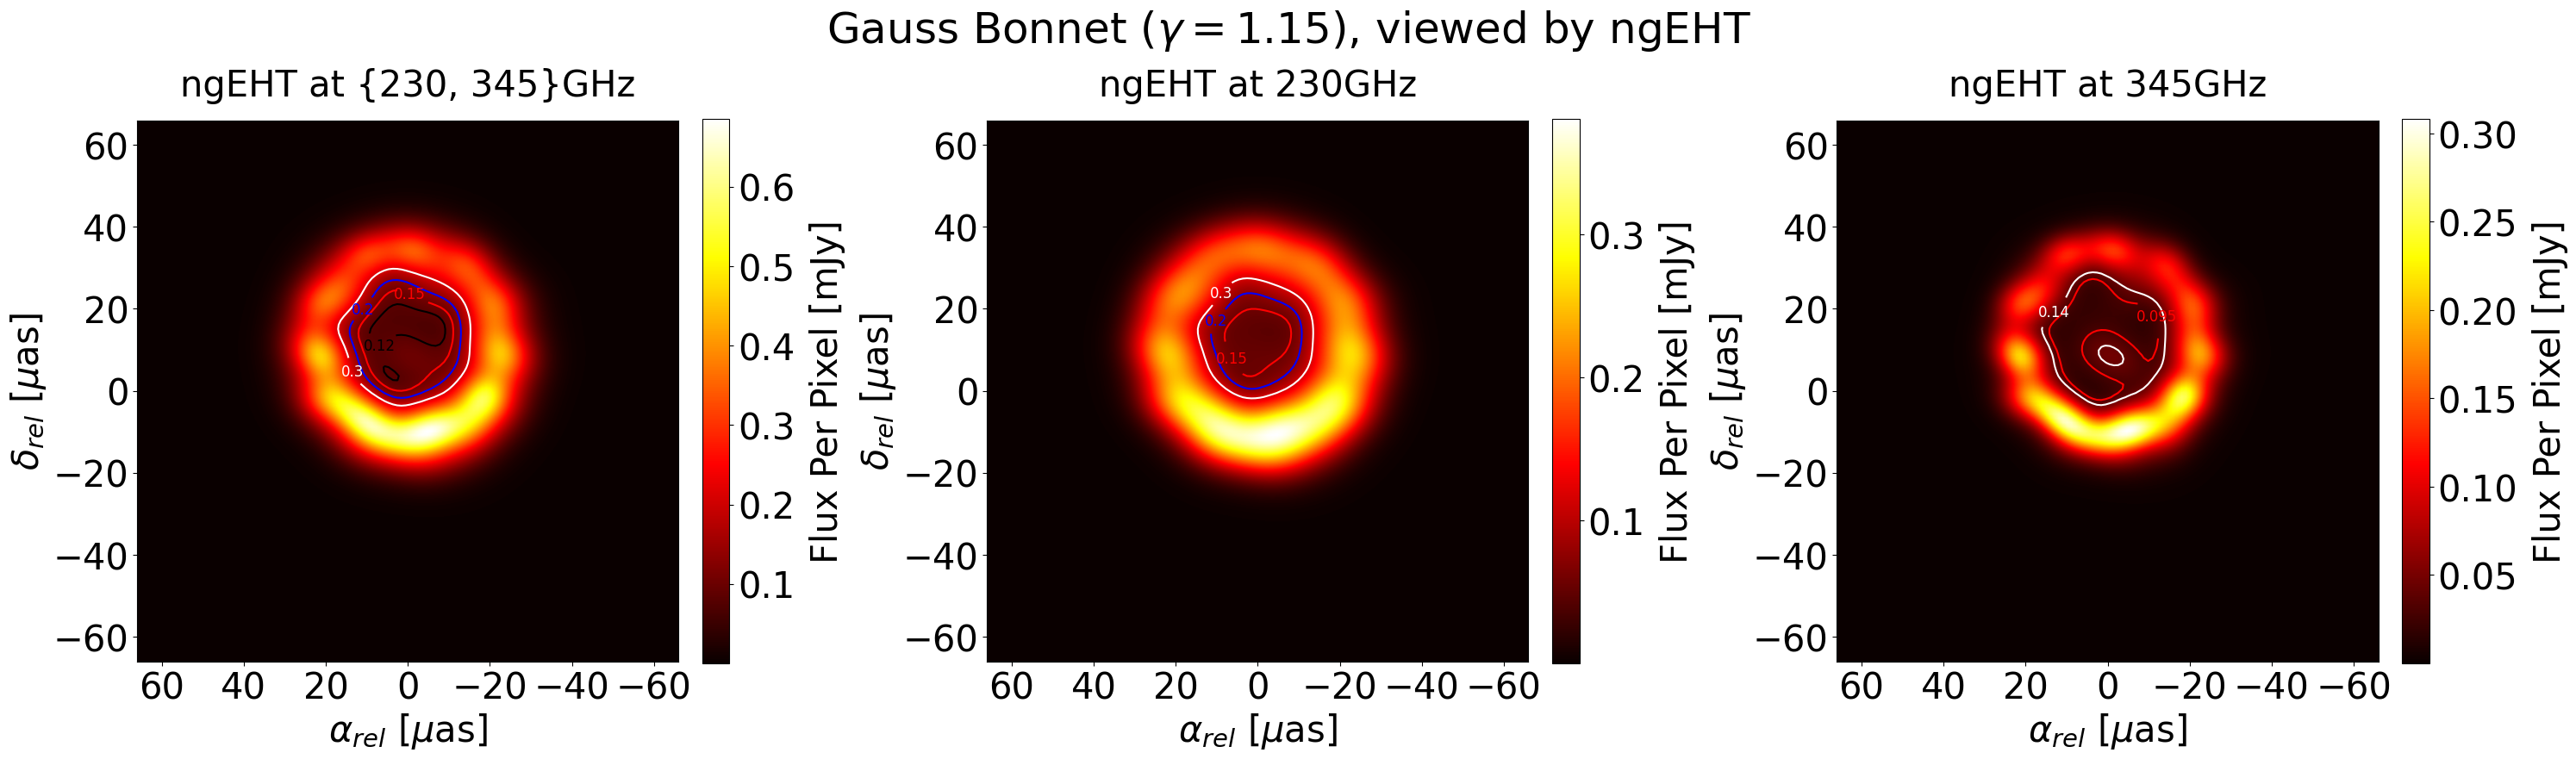
\includegraphics[scale = 0.15]{Pre-Defence/Superpos_Compare_GB.png}
		%\centering
		%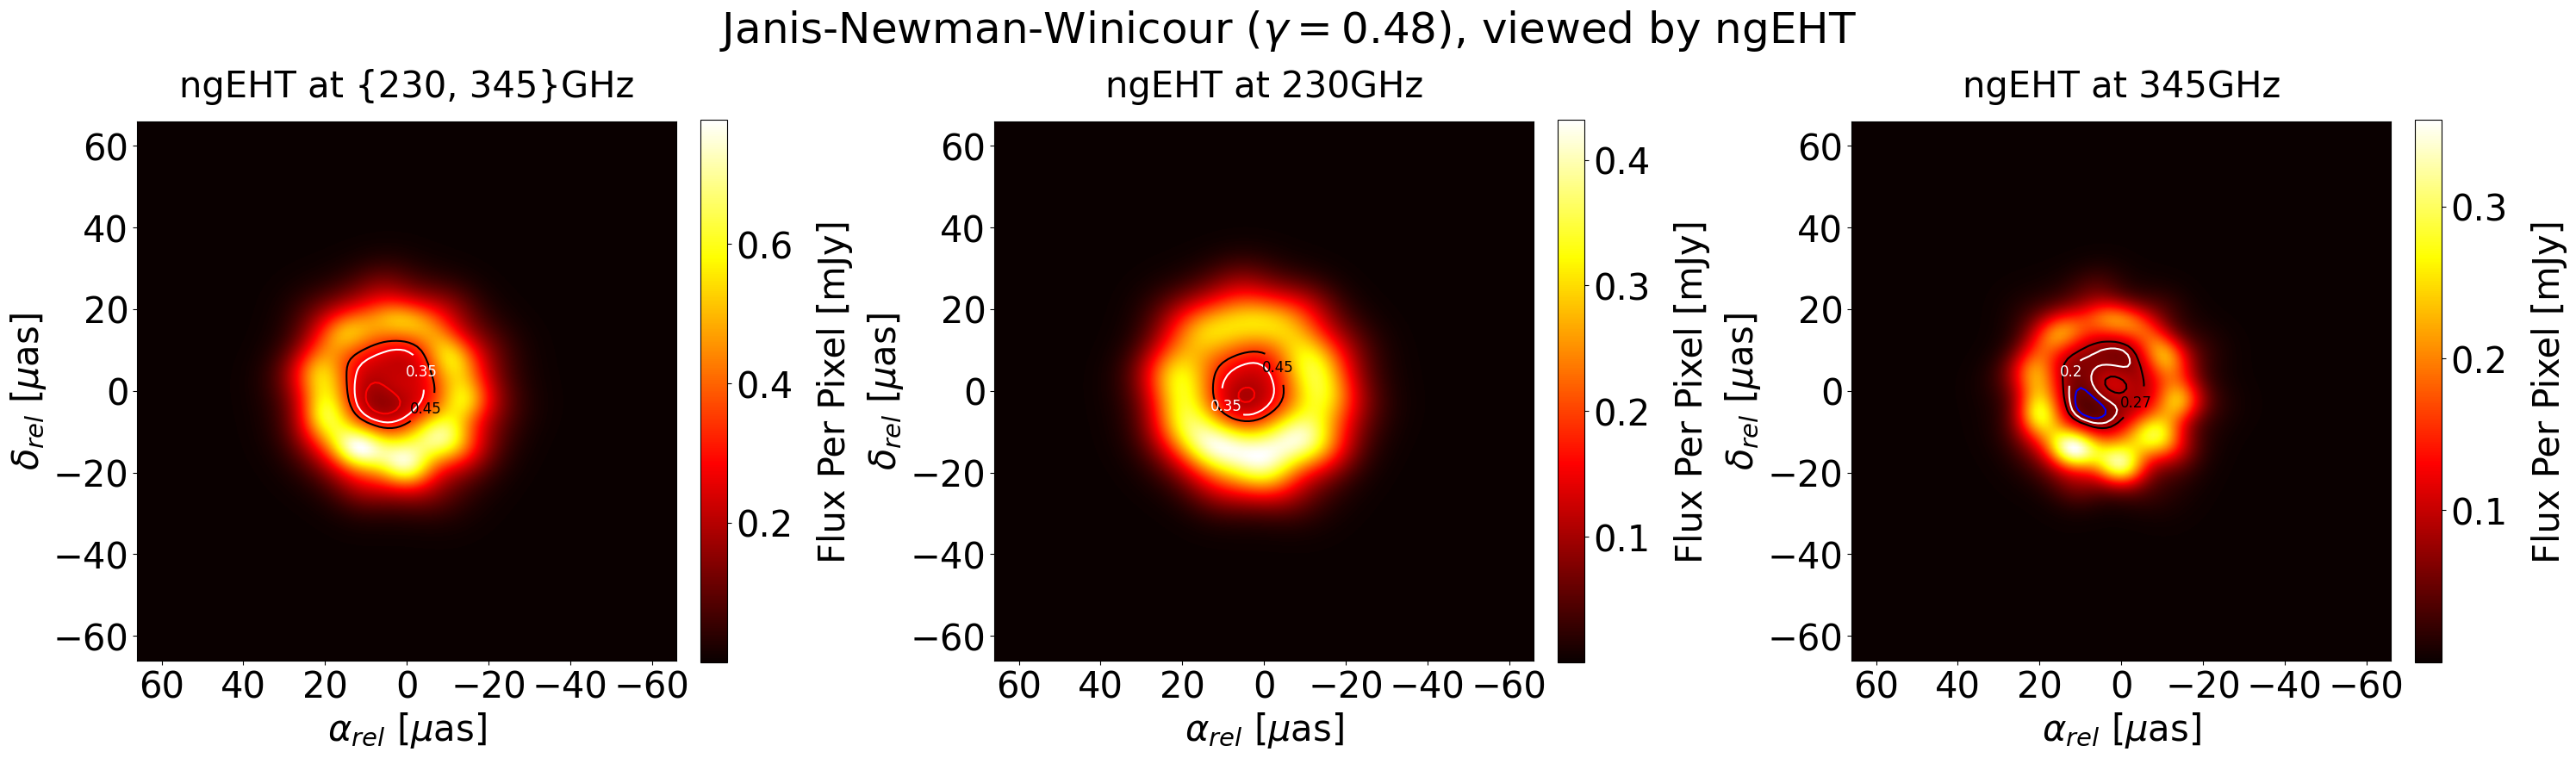
\includegraphics[scale = 0.11]{Pre-Defence/Superpos_Compare_JNW.png}
	\end{frame}
	
	\begin{frame}
		\centering
		Благодаря!
	\end{frame}
	
\end{document}